% This is the Reed College LaTeX thesis template. Most of the work
% for the document class was done by Sam Noble (SN), as well as this
% template. Later comments etc. by Ben Salzberg (BTS). Additional
% restructuring and APA support by Jess Youngberg (JY).
% Your comments and suggestions are more than welcome; please email
% them to cus@reed.edu
%
% See https://www.reed.edu/cis/help/LaTeX/index.html for help. There are a
% great bunch of help pages there, with notes on
% getting started, bibtex, etc. Go there and read it if you're not
% already familiar with LaTeX.
%
% Any line that starts with a percent symbol is a comment.
% They won't show up in the document, and are useful for notes
% to yourself and explaining commands.
% Commenting also removes a line from the document;
% very handy for troubleshooting problems. -BTS

% As far as I know, this follows the requirements laid out in
% the 2002-2003 Senior Handbook. Ask a librarian to check the
% document before binding. -SN

%%
%% Preamble
%%
% \documentclass{<something>} must begin each LaTeX document
\documentclass[12pt, oneside, openright]{byuthesis}


\title{Consistent Mode Choices Across\\
Multiple Model Frameworks}
\author{Christopher Day}
\copyyear{2022}
\committeeMembers{Gregory S. Macfarlane, Chair

Grant G. Schultz

Gustavious P. Williams}
\keywords{four step model, discrete choice model, activity-based model, microsimulation tool, mode choice model, tour purpose, multinomial logit, latent class choice model}
\degree{Master of Science}
\doctype{thesis}
\department{Department of Civil and Construction Engineering}



	\usepackage{algorithm}
\usepackage{algpseudocode}
\usepackage{dsfont}
	\usepackage{booktabs}
\usepackage{longtable}
\usepackage{array}
\usepackage{multirow}
\usepackage{wrapfig}
\usepackage{float}
\usepackage{colortbl}
\usepackage{pdflscape}
\usepackage{tabu}
\usepackage{threeparttable}
\usepackage{threeparttablex}
\usepackage[normalem]{ulem}
\usepackage{makecell}
\usepackage{xcolor}
% End of CII addition
%%
%% End Preamble
%%
%

% Pandoc citation processing
\newlength{\cslhangindent}
\setlength{\cslhangindent}{1.5em}
\newlength{\csllabelwidth}
\setlength{\csllabelwidth}{3em}
\newlength{\cslentryspacingunit} % times entry-spacing
\setlength{\cslentryspacingunit}{\parskip}
% for Pandoc 2.8 to 2.10.1
\newenvironment{cslreferences}%
  {}%
  {\par}
% For Pandoc 2.11+
\newenvironment{CSLReferences}[2] % #1 hanging-ident, #2 entry spacing
 {% don't indent paragraphs
  \setlength{\parindent}{0pt}
  % turn on hanging indent if param 1 is 1
  \ifodd #1
  \let\oldpar\par
  \def\par{\hangindent=\cslhangindent\oldpar}
  \fi
  % set entry spacing
  \setlength{\parskip}{#2\cslentryspacingunit}
 }%
 {}
\usepackage{calc}
\newcommand{\CSLBlock}[1]{#1\hfill\break}
\newcommand{\CSLLeftMargin}[1]{\parbox[t]{\csllabelwidth}{#1}}
\newcommand{\CSLRightInline}[1]{\parbox[t]{\linewidth - \csllabelwidth}{#1}\break}
\newcommand{\CSLIndent}[1]{\hspace{\cslhangindent}#1}

\providecommand{\tightlist}{%
  \setlength{\itemsep}{0pt}\setlength{\parskip}{0pt}}


\begin{document}

\begin{abstract}
Every day individuals make a decision about which modes of transportation they should use. Predicting this behavior perfectly is impossible, however, there are ways to appoximating mode choice in transportation modeling. In this research we aim to increase the accuracy in predicting mode choice using transportation modeling software. Specifically we determine the significance of creating a consistent mode choice model between an activity-based model and a microsimulation tool. Oftentimes, the outputs of an activity-based model serve as the inputs to a microsimulation tool. Yet, the mode choice models betweeen these two software often vary significantly. Using ActivitySim as the activity-based model and BEAM as the microsimulation tool, we establish a consistent mode choice model within BEAM. We then model the mode choice decisions for agents in the Salt Lake City, Utah region. Their modal distributions and mode choice structures are compared to determine the effect of mode choice consistency. Interestingly, we find that a model that uses a consistent mode choice creates a modal distribution that aligns more closely with target shares. We also find that the introduction of path, person, and location variables in the mode choice utility equation helps better predict mode choice decisions. Further research is necessary in order to understand the effects of identical mode choice models between activity-based models and microsimulation tools.
\end{abstract}


\makefrontmatter % this stuff will be roman-numbered
\thesisbody

\hypertarget{introduction}{%
\chapter{Introduction}\label{introduction}}

\hypertarget{problem-statement}{%
\section{Problem Statement}\label{problem-statement}}

The advent of novel transport modes has challenged forecasters to develop new methods of capturing behavior and estimating service capabilities. The usage of bike share, an affordable and sustainable bike rent program, has been modeled countless times each with a different methodology (e.g., Hyland et al. (2018), Biehl, Ermagun, and Stathopoulos (2019), Cho and Shin (2022), W. Li and Kamargianni (2018), Welch, Gehrke, and Widita (2020), X. Zhou, Wang, and Li (2019), Song et al. (2019)). Forecasters are riddled with determining the best technique for understanding who uses e-scooters (public electric scooters) and in what locations they would be most effective (e.g, Zuniga-Garcia et al. (2022), Tuli, Mitra, and Crews (2021), W. Zhang et al. (2021), M. Lee et al. (2021), H. Lee et al. (2021), Hosseinzadeh et al. (2021)). (sentence on e-bikes). In general, forecasters have modeled micromobility (bike share, e-scooters, e-bikes) in many ways, yet few have attempted to model multiple novel modes simultaneously (e.g., Reck et al. (2021), Campbell et al. (2016), Lazarus et al. (2020), McKenzie (2019), Younes et al. (2020)). Ride hail and ride share, which allow users to hire a driver, behave differently than regular car modes. Given their unique nature, understanding their behavior and service capabilities is particularly challenging (e.g., Kang et al. (2021), Y. Li, Liu, and Xie (2020), Dong (2020), Dean and Kockelman (2021)). Forecasters have even attempted to understand the effects of autonomous vehicles, even though to date little to no data exists on fully-autonomous vehicles (e.g., Mo, Chen, and Zhang (2022), Wadud and Chintakayala (2021), F. Zhou et al. (2020)). New transport technologies are becoming more prominent each day, and equally so is the need to accurately capture their behavior.

Various efforts have been made to model novel transport modes accurately, but since methodologies are dissimilar with one another it remains difficult to determine the best approach. For example, some forecasters have chosen to model novel transport modes with an activity-based model, which uses daily activity patterns as the central tool to model an individual's travel behavior (e.g., Xu, Mahmassani, and Chen (2019), Muhammad et al. (2019), Macfarlane, Lant, et al. (2021)). Other forecasters use multi-agent simulation, which focuses on modeling the interactions between different agents, to understand new transport technologies (e.g., Shimizu, Akai, and Nishino (2013), Sánchez et al. (2019), Hörl et al. (2019)). \textbf{Many forecasters have modeled novel modes using a logit based regression analysis, which uses a function to understand characteristics of the modes (e.g., Welch, Gehrke, and Widita (2020), M. Lee et al. (2021), Dong (2020)).}(delete? -- logit regression is used in abm/mas models) Some chose a simpler approach, spatial analysis and geography data, to understand new transport technologies (e.g., Hyland et al. (2018), Cho and Shin (2022), Hosseinzadeh et al. (2021)). Forecasters have even attempted to use machine learning to better understand novel modes! (e.g., X. Zhou, Wang, and Li (2019)). With limited data on novel transport modes, the validity of the results from each approach can be difficult to verify.

\hypertarget{purpose-of-research}{%
\section{Purpose of Research}\label{purpose-of-research}}

In this paper we examine novel mode forecasts generated by different activity-based model and multi-agent simulation mode choice combinations. By examining the ride hail service capabilities between each combination, we hope to understand which mode choice combination is best, or if a best combination even exists. Since only limited data on novel mode usage exists, it seems logical to use a trial and error approach to determine the best way to model new transport technologies. Overall, this paper aims to give forecasters additional direction in how to model novel transport modes.

\hypertarget{literature-review}{%
\chapter{Literature Review}\label{literature-review}}

As discussed in the introduction, forecasters model novel transport modes using activity-based models, multi-agent simulation, spatial analysis, machine learning, and more. Since our research mainly focuses on activity-based models, multi-agent simulation, and the link between them both, understanding the other model frameworks is not within the scope of this project. For this reason, the following literature review outlines the strengths and weaknesses of activity-based models and multi-agent simulation, the previous attempts to model novel transport modes with activity-based models and multi-agent simulation, and the brief literature of those who have attempted to reconcile two modeling approaches within the same study. Within the scope of this paper however, it is not practical to provide a comprehensive review of all activity-based models, multi-agent simulations, or paired modeling approaches.

\hypertarget{lit-abm}{%
\section{Introduction to Activity-based Models}\label{lit-abm}}

Activity-based models are transportation models that construct daily activity patterns from behavioral choice models. They predict what activities are conducted, where those activities are conducted, the length and time of those activities, and the people involved in those activities. This detailed approach to modeling behavior allows forecasters to understand travel at a high level both spatially and temporally. According to Philip, Sreelatha, and George (2013), activity-based models generate travel demand by first modeling activity demand. Understanding the idea that all travel is generated by activities is essential to accurately representing the way people travel. This link between activity and travel allows activity-based models to model behavior especially well, which is particularly advantageous when modeling novel modes. Bowman (1998) also explains that activity-based models have choice models that use utility theory and logit based regression to estimate behavior. These choice models accept an array of inputs relating to person, household, and regional data, to better capture the travel behavior of any particular region.

In addition to representing behavior accurately, another advantage to using activity-based models is that there is modal consistency between trips on the same tour (e.g., Nayak and Pandit (2022), Hasnine and Nurul Habib (2021), Knapen et al. (2021), Gomes, CALDAS, and Pitombo (2021)). Nayak and Pandit (2022) explains that other existing models fail to consider the ``interrelationships among trips'' performed by the same individual on the same tour. For example, if you were to take your car to the gym, and then stop by the store on the way back home, wouldn't you also use your car to get from the store back to your home? Individuals will act similarly among trips of the same tour, and activity-based models account for this natural tendency. Hasnine and Nurul Habib (2021) explains that tour based modeling is the core of activity-based models; ``tackling'' every trip within a tour is essential to understanding the dynamics that exists between trips. Gomes, CALDAS, and Pitombo (2021) explains that trip-based models, unlike activity-based models, disregard trip sequences, trips made by the same individual, and the relationship between trips and activities. Chaining trips of the same individual together, within the same tour, helps ensure modal consistency within models.

Knowing the advantages that activity-based models provide when modeling travel behavior, many forecasters use activity-based models to model the behavior and service capabilities of novel modes. For example, some new technologies that have been modeled with activity-based models are car-sharing (e.g., Nguyen, Hoang, and Vu (2022), Q. Li et al. (2018)) and autonomous vehicles (e.g., Xu, Mahmassani, and Chen (2019), Vyas et al. (2019)). Nguyen, Hoang, and Vu (2022) modeled one-way car-sharing services with an activity-based model because the modal consistency between trips allowed them to track vehicle demand, pricing, and other parameters. Xu, Mahmassani, and Chen (2019) modeled privately-owned autonomous vehicles with an activity-based model as a way to better understand their impact on household travel patterns, including very large households. Macfarlane, Lant, et al. (2021) used an activity-based model to model on-demand wheelchair accessible microtransit vehicles. The activity-based model generated daily activity patterns for all individuals in the region, including those who were wheelchair dependent. With those plans they were able to simulate microtransit vehicles with a microsimulation tool, and process the results to understand service capabilities. Tzouras et al. (2022) conducted a quantitative study of activity-based models for modeling e-scooters. They agreed that activity-based models are an effective vehicle to describe the spatiotemporal variation in e-scooters, and novel modes in general. Muhammad et al. (2019) used an activity-based model to model bike share and even the concept of Mobility as a Service, which aims to make public transport a pay-per-service or monthly subscription. Many forecasters elect to use activity-based models to model new transport technologies because of the behavioral representation and modal consistency they provide.

Although there are advantages to using activity-based models to model novel modes, forecasters must consider the various weaknesses that exist when using activity-based models. One of the biggest shortfalls within most activity-based models is that travel times are averaged along travel links (e.g., RSG (2016), Mahmoudi et al. (2021)). For example, although Nguyen, Hoang, and Vu (2022) used an activity-based models to model one-way car sharing, they noted that it used the BPR function to estimate travel time. The BPR function is a regression function that estimates average travel time based on arrival flows. When using the BPR function to estimate smaller time intervals though, it becomes inconsistent. For this reason, Nguyen, Hoang, and Vu (2022) noted that it was more difficult to verify the service capabilities of the car-sharing modes. Similarly, on-demand microtransit vehicles should be modeled with variable wait time; the difference between a 4 minute wait and a 17 minute wait is significant when traveling. Macfarlane, Lant, et al. (2021) recognized this shortcoming, and elected to estimate the on-demand travel time by using a multi-agent simulation on top of an activity-based model. Overall, since travel time is a significant part of the mode choice utility, average travel time is a shortfall when modeling novel modes.

Another typical weakness present in most activity-based models is their focus on individual-based behavior, instead of household-based behavior. Although it is widely known that many decisions made by humans are done collectively, little effort has been made to model travel based on intra-household interactions and group decisions making (J. Zhang and Fujiwara 2006). However, some forecasters have attempted to account for this shortfall (e.g., J. Zhang and Fujiwara (2006), Neutens et al. (2008), Soo (Kum Lin (2009)). Neutens et al. (2008) and Soo (Kum Lin (2009) in particular attempted to extend individual-level travel to household-level travel by assigning certain tasks (activities) to different household individuals, verifying that schedules within the same households were coherent, and developing a household utility measure. J. Zhang and Fujiwara (2006) developed a household utility function to help represent the ``diverse intra-household interactions''. Travel behavior is more than just a set of strung together activities, and certain interactions (e.g., household-based decisions) are important to consider when modeling transport modes.

\hypertarget{lit-mas}{%
\section{Introduction to Multi-agent Simulation}\label{lit-mas}}

An alternative to activity-based models for forecasting novel modes is multi-agent simulation. Multi-agent simulation, usually synonymous with the term microsimulation, models interactions between individual agents. Multi-agent simulation is a desirable tool because it allows analysis to be done on both the individual and group levels; individualized decisions can be explored (e.g., Kamel et al. (2019)) as well as agent to agent interactions (e.g., Bazghandi (2012), Amblard et al. (2015), Siebers and Aickelin (2008)). These agent to agent interactions and individualized decisions allow forecasters to better understand why a novel mode may or may not be chosen. For example, multi-agent simulation allows forecasters to know exactly how many users participate in a novel transport mode, which type of users are interested in a novel transport mode, and if other agents played a role in the novel transport mode choice decision.

Along with modeling unique agents, another reason multi-agent simulation is advantageous for modeling novel modes is its transportation network and capacity constraint. Transportation networks are visual representations of the actual road networks, and allow forecasters to see the transportation decisions made by each agent. In addition to being visual tools, agents are coded to the network allowing them to interact with attributes of the network itself. For example, Dia (2002) used a real traffic network in their model to simulate areas of high traffic congestion. Within the model, agents could notice high congestion areas and some of them would chose to take an alternate route. Due to the interaction between individual agents and roadway conditions, realistic travel behavior is captured on a global scale. Djavadian and Chow (2017) and Fujii, Uchida, and Yoshimura (2017) also used a real transportation network to capture realistic global travel behavior. Djavadian and Chow (2017) explored the usage of flexible mobility systems like taxi and carpool and Fujii, Uchida, and Yoshimura (2017) explored mixed traffic consisting of cars, pedestrians, and trams. Fujii, Uchida, and Yoshimura (2017) even enhanced the basic transportation network system by coding various virtual driving lanes at each intersection, thus making the network even more realistic. Cetin et al. (2002) describes two more benefits of road networks: one, vehicles are subject to remain on network links for a certain amount of time (according to their travel speed) and, two, a storage capacity exists for each link that once met, no more vehicles can enter. By using a transportation network, the travel times, speeds and congestion become reliable model outputs, and therefore, the travel times, speeds, and congestion of novel modes are easily modeled. Multi-agent simulation uses unique agents with a realistic transportation network to create attainable and reliable model outputs.

Due to the advantages that multi-agent simulation provides, various forecasters have elected to use them to model novel transport modes. For example, Kamel et al. (2019) chose to use a multi-agent simulation to model shared autonomous vehicles because decision-making was done on an individual level. This granularity helped the researchers understand how user preferences affected the modal split of shared autonomous vehicles. Hörl et al. (2019) also analyzed shared autonomous vehicles with a multi-agent simulation, mainly to take advantages of the detailed network dynamics. By utilizing the detailed network, the researchers were able to estimate the system performance, wait times, and cost of various autonomous vehicle fleets. Other analyses have been completed on other novel modes like with shared mobility (e.g., Ciari, Balac, and Axhausen (2016), Shimizu, Akai, and Nishino (2013), Becker et al. (2020)) and electric vehicles (e.g., Sánchez et al. (2019)). Specifically, Ciari, Balac, and Axhausen (2016) summarizes a multitude of research done to understand demand for car-sharing with the multi-agent simulation model MATSim. In this research, they note that although multi-agent simulation provides an extensive level of detail, it does not necessarily equate to real world accuracy. A model rich in detail and with extensive behavioral rules, however, allows innovative transportation technologies to be analyzed efficiently in a world where ``solid behavioral knowledge does not yet exist''. Therefore, by using MATSim, Ciari, Balac, and Axhausen (2016) surpassed the typical pitfalls of modeling a new transport mode like car-sharing, and adequately modeled the individual travel decisions with a high temporal and spatial resolution. Similarly, Becker et al. (2020) used MATSim to model different shared mobility services (car-sharing, bike-sharing, ride-hailing). By using a multi-agent simulation, multiple novel transport modes could be analyzed simultaneously within the same model. Many forecasters continue to analyze new transportation technologies with multi-agent simulation because its inherit advantages are helpful to understanding service capabilities.

Although the advantages within multi-agent simulation are useful to modeling novel modes, forecasters must be aware of the weaknesses within these models as well. For example, although Kamel et al. (2019) used multi-agent simulation to model shared autonomous vehicles, they understood that the homogeneous behavior structure may decrease the accuracy of their results. A homogeneous behavior structure means that all agents within the model have similar preferences when facing decisions, like mode choice. This renders results to be less accurate since oftentimes people choose a specific mode based solely on their personal preference. Tchappi et al. (2018) reviews many of the advantages of a holonic multi-agent simulation (holonic meaning to divide the system into dependent groupings), but acknowledges the weakness that driver behavior is not homogeneous. The other major weakness of multi-agent simulations is their high computational requirements (e.g., Siebers and Aickelin (2008), Cetin et al. (2002), Adler et al. (2005)). In order to adequately model the individualized nature of every agent, while mapping each agent to a detailed road network, affluent computing power is needed. The need for a high processing computer and sufficient computing time is indeed a limitation for some forecasters.

Another inherit weakness of most multi-simulation models is its focus on trips-based modeling. Most multi-simulation models only simulate agents on a trip level, ignoring the tour-based framework present in most activity-based models. Figure \ref{fig:fig-mode-compare} provides a visual example of this difference. If a person wants to go to their work activity by train, an activity-based model knows that they can either walk or take transit to their gym activity. Contrastingly, a multi-agent simulation bases mode choice on the first trip of the day. This means that a multi-agent simulation will determine the optimal mode to go to the gym in, and then figure our how to get to work based on the first trip mode. In addition, an activity-based model knows that when a person leaves for lunch from their work activity, they will be returning back to their work activity after lunch. This means that the person is able to leave their car at work and possibly walk or take transit to and from their lunch activity. In a multi-agent simulation though, if someone goes to lunch, they will most likely take their car as to not abandon their vehicle for the rest of their day. It is clear that a multi-agent simulation's mode choice is less representative of how people actually transport themselves during the day. An activity-based model provides a better representation of mode choice. In this research we attempt to link a activity-based model and a multi-agent simulation tool as to use the advantages of both models to better model novel transport modes.

\begin{figure}

{\centering 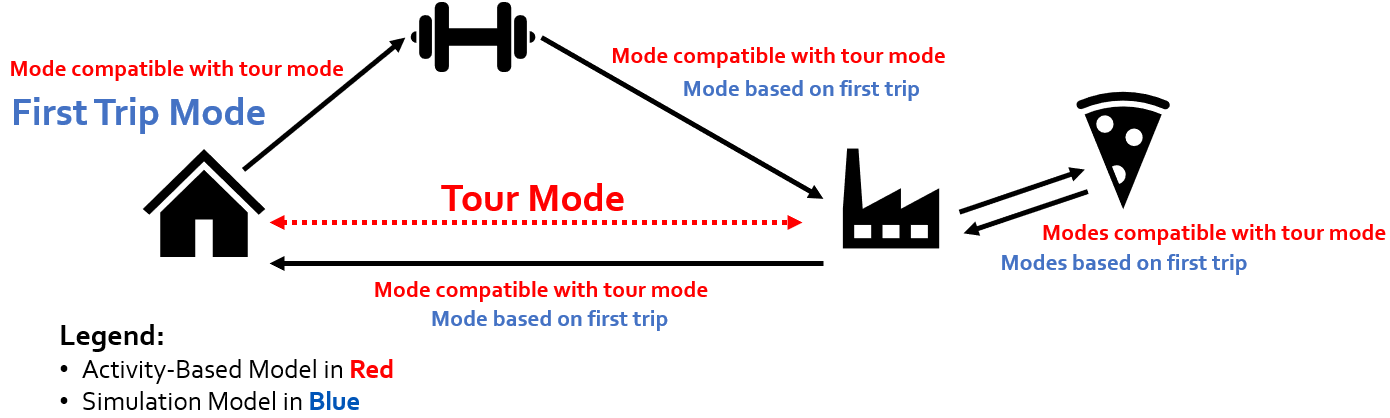
\includegraphics[width=1\linewidth]{pics/abm-mas-compare} 

}

\caption{Mode Choice in Activity-based Models and Multi-agent Simulation.}\label{fig:fig-mode-compare}
\end{figure}

\hypertarget{limited-attempts-to-pair-two-disparate-modeling-approaches}{%
\section{Limited Attempts to Pair Two Disparate Modeling Approaches}\label{limited-attempts-to-pair-two-disparate-modeling-approaches}}

The varying strengths and weaknesses within both activity-based models and multi-agent simulation point to possibly using both approaches to understand novel mode behavior. Yet few forecasters have attempted to reconcile or pair these two disparate approaches in order to better understand novel mode behavior. However, one example of reconciling the traditional approaches is with the system MITO (e.g., Moeckel et al. (2020), Zwick et al. (2021)). MITO stands for Microsimulation Transport Orchestrator, and its primary purpose is to overcome the limitations of the traditional trip-based model while being easier to implement than the traditional activity-based model. Like a multi-agent simulation, MITO simulates each agent individually, however, MITO also restricts agents of the same household with a travel time budget. This travel time budget influences destination choice, and ensures that agents participate in sensible activities (e.i. those household members who commute to work are less likely to perform shopping and discretionary activities). MITO includes a simplified activity schedule builder, allows forecasters to add attributes, allows agent tracing, and is not as computationally heavy as traditional multi-agent simulations (Moeckel et al. 2020). Zwick et al. (2021) used MITO to estimate travel demand and MATSim, a multi-agent simulation tool, to simulate that demand. By pairing together MITO and MATSim, the researchers were able to gather service criteria for a novel transport mode: pooled on-demand ride hailing vehicles.

Traditionally, MATSim implements a feedback loop to determine mode choice instead of using a discrete choice model. For example, if in one iteration too many agents choose a car mode and travel times go up, in the next iteration some agents will opt to use an alternative mode. This process continues until equilibrium is found between the supply and demand. Some researches have attempted, however, to pair together a discrete mode choice models with MATSim in attempt to shorten the number of iterations needed to be run. For example, Hörl, Balać, and Axhausen (2019) discovered that by using a discrete choice model within MATSim, no irrelevant mode choice decisions were made. This indeed, lead to less iterations being run. However, although initial modal decisions were more accurate than the default MATSim model, the discrete choice model added a layer of complexity. Accurate and consistent data is needed in order for the discrete choice model to work effectively. This need for more data gives the model runners less freedom. Hörl, Balać, and Axhausen (2019) mentions that their research was merely an introduction to the concept, and further research is desirable to understanding all the benefits of linking discrete choice and simulation based tools.

Another example of pairing together two different modeling approaches is with an activity-based model and a dynamic traffic assignment model (e.g., L. Zhang et al. (2018), Pendyala et al. (2017), Shiftan (2000)). Dynamic traffic assignment models are useful as they understand time-dependent interactions, simulate individual agents, capture congestion, and can model new transportation technologies (L. Zhang et al. 2018). Pairing together activity-based models and dynamic traffic assignment models is of great interest to forecasters, as their structures are similar and together they produce results at a finer level of detail. L. Zhang et al. (2018) paired together InSITE, an activity-based model, with DTALite, a dynamic traffic assignment model, to model travel demand in the Baltimore-Washington region. Their conclusion was that the integrated model performed better than the singular InSITE activity-based model. Overall, they determined that the integrated model produced better results, but was more challenging to run and required consistent upkeep to ensure consistency between models.

To the authors knowledge, no previous literature exists on pairing together an activity-based model with a multi-agent simulation for the purpose of modeling novel mode behavior. Yet both activity-based models and multi-agent simulation have their own unique strengths when it comes to modeling novel modes. Could using both an activity-based model and a multi-agent simulation within the same study maximize each model's strengths while limiting each model's weaknesses? There exists a need to understand which methodology is best for modeling novel modes, or if a best methodology even exists. The objective of this study is to better understand the effects of using different mode choice combinations between varying activity-based models and multi-agent simulation combinations. We aim to use these results to provide forecasters guidance as to which choice model combination they should use to model novel modes.

\hypertarget{methods}{%
\chapter{Methods}\label{methods}}

We developed a series of experiments to understand the relative importance of activity-based and multi-agent simulation in forecasting the uptake of novel modes. These experiments were performed using ActivitySim as the activity-based model and BEAM as the multi-agent simulation tool. We used the Salt Lake City, Utah region as a case study for our experiments. Since ride hailing vehicles were an emerging technology in the region at the time of our study, we deemed it the appropriate novel transport mode to model in our experiments. The following section outlines the methodology for which we were able to model a novel transport mode with differing activity-based model and multi-agent simulation mode choice combinations.

\hypertarget{meth-asim}{%
\section{ActivitySim as the Activity-based Model}\label{meth-asim}}

ActivitySim is an activity-based simulator used to generate plans for millions of agents each with their own demographic attributes (Gali et al. 2008). Instead of independently modeling each trip, ActivitySim simulates each individual by calculating their daily travel diaries and schedules. Long term decisions are made first, and then shorter term decisions are calculated based on those long term decisions ({``ActivitySim: An Advanced Activity-Based Travel Demand Model Built by and for Users''} 2021). Overall, ActivitySim is an advanced activity-based model with the same advantages and disadvantages described in Section \ref{lit-abm}.

\hypertarget{novel-modes-in-activitysim}{%
\subsection{Novel Modes in ActivitySim}\label{novel-modes-in-activitysim}}

ActivitySim was chosen as the activity-based model in this research because built into its framework are the novel modes of ride hail and pooled ride hail. Specifically, ride hail and pooled ride hail fall under one of the four nested tiers of ActivitySim's nested logit model. This means that ride hail is a unique modal option not characterized by being an auto, non-motorized, or transit type mode. Figure \ref{fig:fig-asim-nest} displays the four tiers of the nested logit along with the modal alternatives of each tier (MTC 2012). These modal alternatives represent the alternatives available in both ActivitySim's tour based and trip based mode choice model. When determining the mode to use on a trip, ActivitySim first calculates the tour mode and subsequently calculates the trip mode based on the tour mode selection (See Figure \ref{fig:fig-mode-compare}). Person attributes, path attributes, location attributes, tour purpose value, and more all play a role in calculating the mode choice decision.

\begin{figure}

{\centering 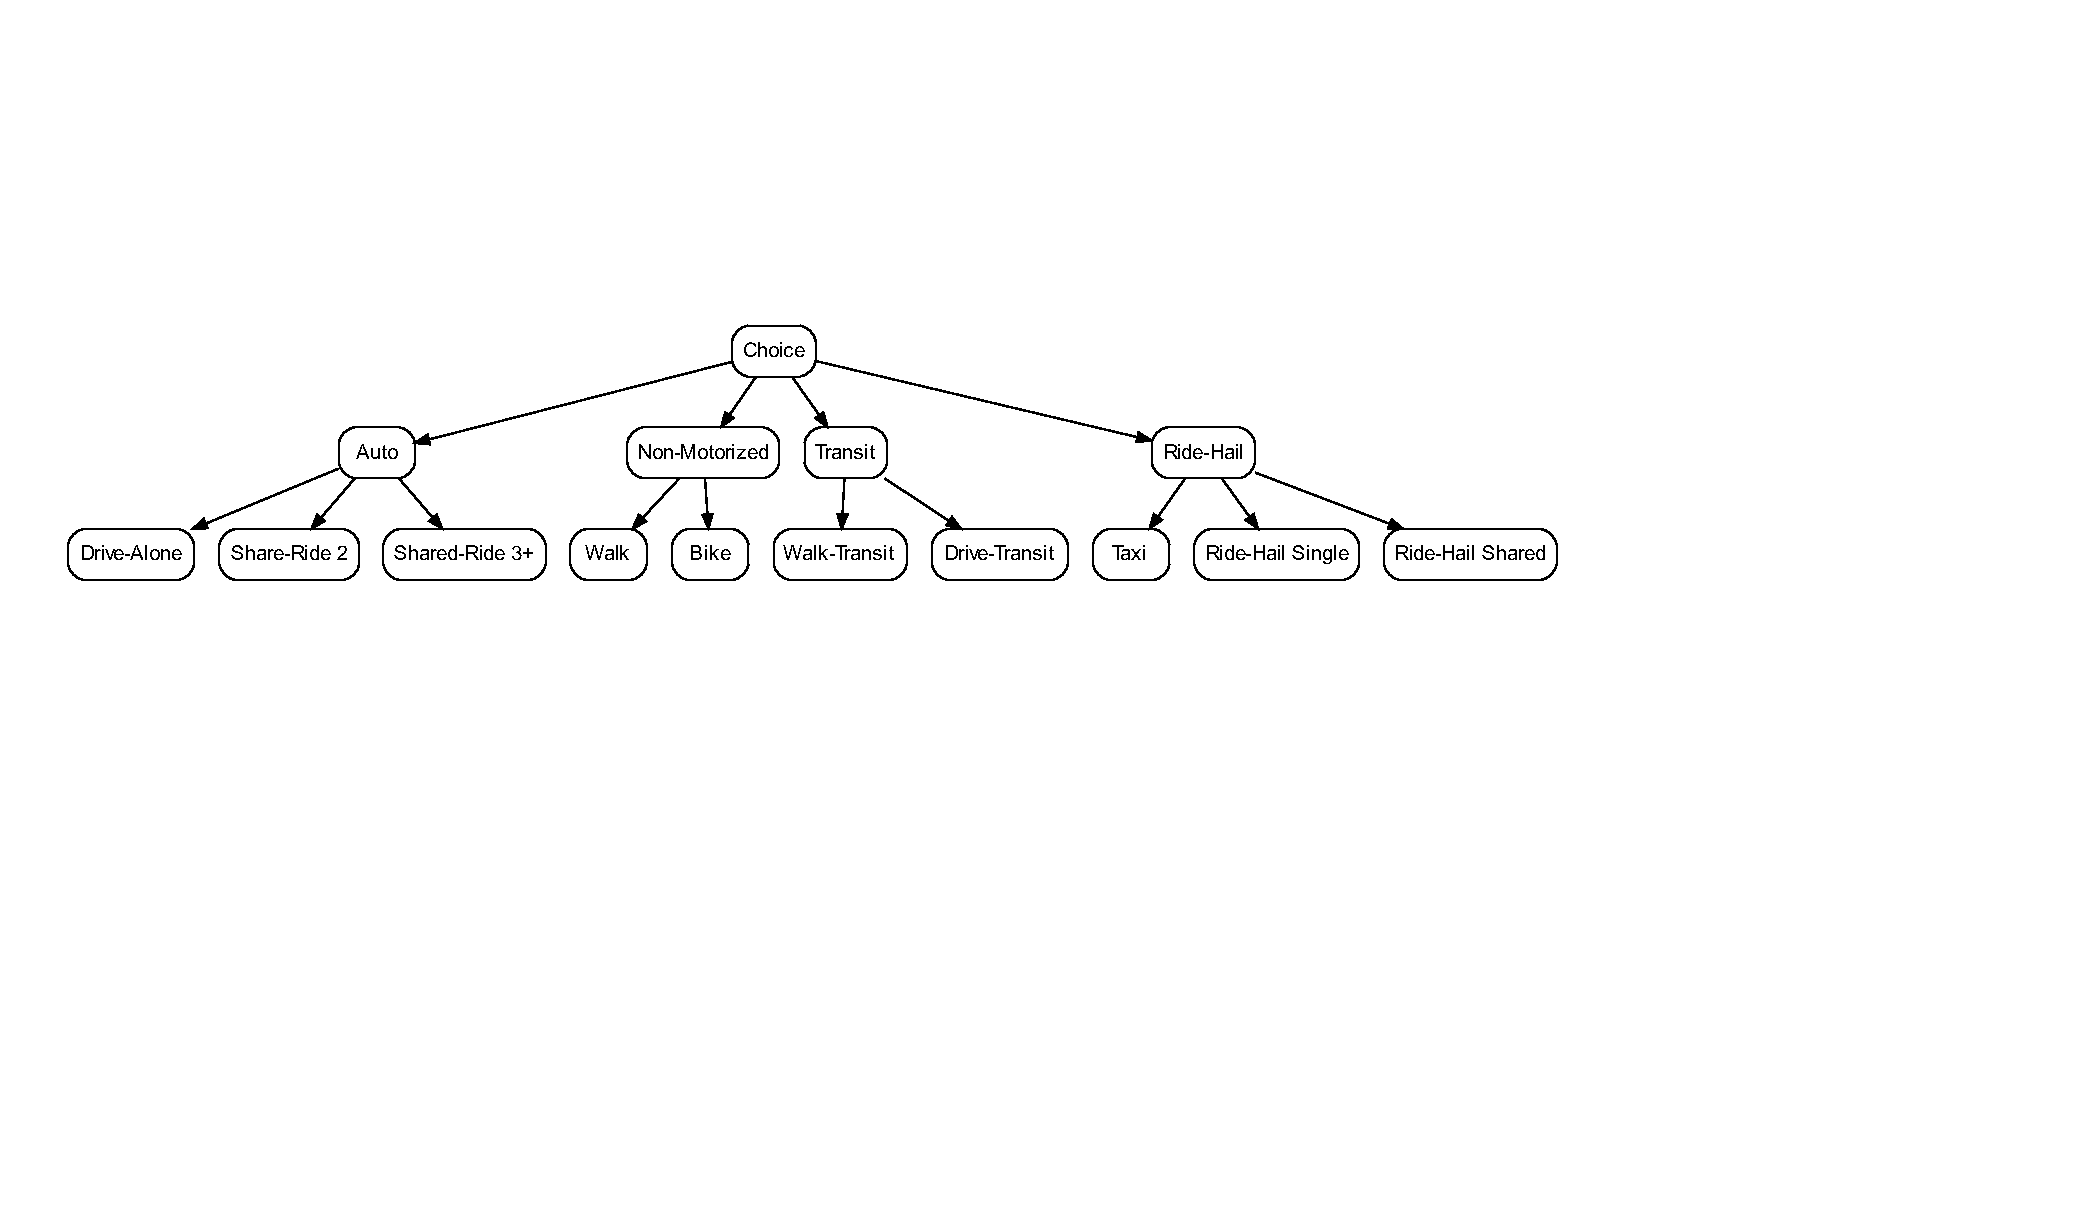
\includegraphics[width=.7\textwidth,trim = {5cm 6.5cm 12.5cm 4cm}]{thesis_files/figure-latex/fig-asim-nest-1} 

}

\caption{ActivitySim Nested Logit Model.}\label{fig:fig-asim-nest}
\end{figure}

In addition to using specific attributes to determine the mode choice decision, ActivitySim also sets default parameters for choosing ride hail and pooled ride hail vehicles. For example, a base fare, cost per mile, cost per minute, and cost minimum are all set before model runs. These values can be changed between model runs, but are held constant for all ride hail vehicles in the same model run. In addition, a mean wait time is used to help calculate the total travel time of ride hail vehicles. This means that all mode choice decisions to choose ride hail vehicles use the same wait time in the utility calculation. There is no variability in wait time between one agent using ride hail against another. One exception however, is that there are 5 different mean wait time values depending on the location of the ride hail request. Mean wait times also differ between single ride hail trips and shared ride hail trips. There is also one parameter for the maximum allowed wait time for a ride hail vehicle. Overall, it was essential to use ActivitySim to model ride hail vehicles because the mode choice structure fostered accurate behavioral representation and modal consistency between trips. However, ActivitySim's absence in using variable wait time to calculate the ride hail choice utility led us to also modeling ride hail vehicles with a multi-agent simulation (See Section \ref{meth-beam}).

\hypertarget{activitysim-configured-to-the-case-study-region}{%
\subsection{ActivitySim Configured to the Case Study Region}\label{activitysim-configured-to-the-case-study-region}}

ActivitySim was configured to the case study region by first gathering and generating the input data. Three input files were necessary in order to run ActivitySim:

\begin{enumerate}
\def\labelenumi{\arabic{enumi}.}
\tightlist
\item
  A synthetic population of the agents within the study area.
\item
  A zonal socioeconomic data file describing the characteristics of each zone.
\item
  A set of skims that describe the cost and travel times of all modes between all zones.
\end{enumerate}

A synthetic population is a generated population with specific individual attributes that add up to the regional characteristics as a whole. We generated the synthetic population using a software called PopulationSim (PopulationSim 2021). We used a ``seed'' table, which represented information of a subset of the population, and a set of ``targets'', which represented demographic data of smaller areas of the region, to run PopulationSim (Lant 2021). The zonal socioeconomic data file stores zonal characteristics regarding household, worker, and other activity type information. This file was created using data from Wasatch Front Regional Council (WFRC) (WFRC 2019), Utah Automated Geographic Reference Center (AGRC 2021), and the synthetic population when necessary. The skims are large matrices showing travel times and costs between every set of zones within the area of study. Included in these skims were further details regarding differences in modes, distances, wait times, etc. (Lant 2021). We used pre-generated skims from WFRC (2019), with some slight adjustments, in our run of the ActivitySim model.

After generating the necessary input files, we calibrated and validated the ActivitySim model to better represent decisions made in the Salt Lake region. The process of calibrating and validating the ActivitySim model to the Salt Lake region was conducted by Lant (2021). The purpose of the calibration and validation was to ensure that the outputs generated by ActivitySim matched target regional values. Specifically, trip productions, trip distributions, and mode choices were tested to match the given target values from the four-step model from WFRC (2019). The details behind the exact calibration and validation process are discussed by Lant (2021), and therefore will not be described in detail within this paper. However, we did conduct one additional calibration measure beyond that which Lant (2021) completed. Due to some slight adjustments made after the initial calibration of ActivitySim, we elected to re-calibrate ActivitySim's tour mode choice parameters. Using the 2012 household travel survey as our targets, we improved ActivitySim to model a more accurate total modal distribution of the region (WFRC 2019). The fully calibrated and validated ActivitySim model was then ready to run and generate activity plans for the case study region.

\hypertarget{meth-beam}{%
\section{BEAM as the Multi-agent Simulation Tool}\label{meth-beam}}

BEAM stands for Behavior, Energy, Autonomy, and Mobility and is a multi-agent simulation tool being developed by Lawrence Berkeley National Laboratory and UC Berkeley Institute for Transportation Studies (BEAM 2022). As an extension of MATSim, it simulates individual agents using both within day replanning and across-day replanning to maximize individual utility. Overall, BEAM shares many of the same advantages and disadvantages of most multi-agent simulations as described in Section \ref{lit-mas}.

\hypertarget{novel-modes-in-beam}{%
\subsection{Novel Modes in BEAM}\label{novel-modes-in-beam}}

BEAM was chosen as the multi-agent simulation in this research because of its integration with transportation network companies (TNCs), or ride hail and pooled ride hail vehicles. (BEAM also supports plug-in electric vehicle modeling, however, this feature was not used within our research.) Along with the TNC type mode options, BEAM supports many of the regular choices as well, such as car, walk, bike, walk-to-transit, and drive-to-transit. Default BEAM uses a simple multinomial logit choice model for determining which mode any particular agent will use on any particular trip. Only a few variables are used to calculate the modal alternative: cost, travel time, number of transfers, and an alternative specific constant (ASC) (BEAM 2022).

BEAM was also chosen as the multi-agent simulation in this research because of how it implements ride hailing vehicles. BEAM uses a greedy asynchronous ride hail matching algorithm that also supports pooled trips. The algorithm works by first, requiring agents to send a request for a ride hail vehicle, and then by second, matching the closest vehicle to that agent. For the algorithm to work, BEAM requires the modeler to input a ride hail vehicle fleet. This fleet is a simply file that describes the number of ride hailing vehicles available in the region, their starting locations, their working hours, their seating capacity, and other specifications. BEAM assigns these vehicles to the roadway network, where they ``roam'' the streets awaiting requests. The ride hail algorithm permits a more realistic ride hail modeling structure. For example, agents make a request to take a ride hail vehicle, expect a variable wait time dependent on their geographic location, and may not even be able to take the vehicle if there is no availability! All these attributes are similar to how using ride hail is in real life, and represent the true advantages to modeling ride hail with BEAM.

\hypertarget{meth-beam-link}{%
\subsection{Linking the Mode Choice of ActivitySim and BEAM}\label{meth-beam-link}}

In order to use BEAM in conjunction with ActivitySim, however, its mode choice model was updated to be more consistent with ActivitySim's mode choice model. More specifically, three changes were made to the choice structure:

\begin{enumerate}
\def\labelenumi{\arabic{enumi}.}
\tightlist
\item
  Adding a Tour Purpose Attribute
\item
  Adding Person, Path, and Location Attributes to the Utility Equation
\item
  Adding New Modal Alternatives
\end{enumerate}

First, a tour purpose attribute was added at the trip level, to be used when making trip-based modal decisions. ActivitySim's default utility parameters are segmented by tour purpose, auto ownership, and mode; therefore, adding a tour purpose level attribute was essential to calculating the mode choice utility similar to ActivitySim.

Second, multiple person, path, and location related attributes were added to use in the mode choice utility equations. The MTC example of Activityim (the example referenced in this research) uses 25 different variables in the utility calculation (MTC 2012). So, BEAM was adjusted to use values like wait time, transit proximity, distance, age, household size, and more on top of the default variables to calculate modal utility. This was done by gathering path and location variables from the BEAM router and person level variables from the input files. ASCs were copied directly from the MTC ActivitySim example, and then calibrated later on. Overall, one input file was created which housed all path, person, and location type parameters on a tour purpose, auto ownership, and modal level.
The last major adjustment made to the BEAM software was adding new modal alternatives. The most important difference between the ActivitySim modal options and the BEAM modal options is the inclusion of carpooling vehicles (HOV2 and HOV3). HOV2 means High Occupancy Vehicle with 1 passenger (2 people in the vehicle) and HOV3 means High Occupancy Vehicle with 2 or more passengers (at least 3 people in the vehicle). The BEAM software was adjusted to include HOV2 and HOV3 type modes, including a distinction between drivers and passengers of those vehicles. Within the code, HOV2 and HOV3 modes were provided as modal options by transforming an existing car option into an HOV option. This allowed car travel statistics to be transferred over to the carpooling modes, which were essential to calculating the utility.

BEAM's default mode choice model was adjusted dramatically to be more closely aligned with how the MTC example of ActivitySim handles mode choice (MTC 2012). As a way to better understand the complexity of the new mode choice model in BEAM, two pseudocode algorithms are provided. Specifically, the algorithms are meant to provide clarification on how BEAM's new mode choice model works.

Algorithm 1 describes the process behind determining the mode choice alternatives for each agent. This process occurs for every agent for every trip. Two procedures are presented within the first algorithm. The first procedure is called DetermineHOVAlternatives. This procedure was added to the BEAM code as a way to include carpooling options. In this procedure the HOV alternatives are created from already existing options created by the R5 router (Conveyal 2022). (The R5 routing engine helps BEAM accomplish multi-modal routing). Basically if a car, HOV2, or HOV3 mode is already created from the router, then both HOV2 and HOV3 options are provided. If car is not provided by the router, then passenger HOV options are provided. Passenger HOv modes, called HOV\_TELEPORT, are completed by teleporting agents from origin to destination. The second procedure within Algorithm 1 describes the process behind determining the final modal alternatives. It essential states that if the current mode is already chosen, then that mode remains as the only alternative to choose from. However, if no mode is currently chosen for the trip, the router, ride hailing, and HOV alternatives are combined and presented as the final alternatives to choose from.

\begin{algorithm} [tph]
\caption{Algorithm for Determining Mode Choice Alternatives in BEAM}
\begin{algorithmic}[1]
\Require
\State $i : origin$
\State $j : destination$
\State $n: agent$
\State $N: population$
\State $t : trip $
\State $P : plan$
\State $\vec{R}(i,j) : Router\: alternatives$
\State $\vec{RH}(i,j) : Ridehail\:alternatives$
\State $\vec{H}(i,j) : HOV\:alternatives$
\State $\vec{M}(i,j) : Final\:modal\:alternatives$
\State $C : Current\:Mode$
\State $I : Trip\:Index$
\vspace{4pt}\hrule\vspace{5pt}

\State $\vec{R} \equiv \vec{R}(i,j)$
\State $\vec{RH} \equiv \vec{RH}(i,j)$
\State $\vec{H} \equiv \vec{H}(i,j)$
\State $\vec{M} \equiv \vec{M}(i,j)$
\For {$n \in N$}
\For {$t \in P$}

\Procedure {DetermineHOVAlternatives}{$\vec{R}$, $C$}
\If {$C=None$}
  \If {$\vec{R} \ni CAR$}
    \State $\vec{H} \gets (HOV2,HOV3)$
  \ElsIf {$\vec{R} \ni HOV2$}
    \State $\vec{H} \gets (HOV3)$
  \ElsIf {$\vec{R} \ni HOV3$}
    \State $\vec{H} \gets (HOV2)$
  \ElsIf {$\vec{R} \ni WALK$}
    \State $\vec{H} \gets (HOV2\_TELEPORT, HOV3\_TELEPORT)$
  \EndIf
\Else
  \State $\vec{H} \gets None$
\EndIf
\EndProcedure
\Statex
\algstore{myalg}
\end{algorithmic}
\end{algorithm}

\addtocounter{algorithm}{-1}
\begin{algorithm}
\caption{continued}
\begin{algorithmic} [1]
\algrestore{myalg}
\Procedure {DetermineFinalModalAlternatives}{$\vec{R}$, $\vec{RH}$, $\vec{H}$, $C$, $I$}
\If {$C = DRIVE\_TRANSIT \lor BIKE\_TRANSIT$}
  \If {$I = 0$}
    \If {$C = DRIVE\_TRANSIT$}
      \State $\vec{M} \gets (DRIVE\_TRANSIT)$
    \Else
      \State $\vec{M} \gets (BIKE\_TRANSIT)$
    \EndIf  
  \Else
    \State $\vec{M} \gets (WALK\_TRANSIT, RIDEHAIL\_TRANSIT)$
  \EndIf
\ElsIf {$C = WALK\_TRANSIT \lor RIDEHAIL\_TRANSIT$}  
  \If {$C = WALK\_TRANSIT$}
    \State $\vec{M} \gets (WALK\_TRANSIT)$
  \Else
    \State $\vec{M} \gets (RIDEHAIL\_TRANSIT)$
  \EndIf
\ElsIf {$C = HOV2\_TELEPORT \lor HOV3\_TELEPORT$}  
  \If {$C = HOV2\_TELEPORT$}
    \State $\vec{M} \gets (HOV2\_TELEPORT)$
  \Else
    \State $\vec{M} \gets (HOV3\_TELEPORT)$
  \EndIf
\ElsIf {$C = CAR$}
  \State $\vec{M} \gets (CAR)$
\Else
  \State $\vec{M} \gets \vec{R} + \vec{RH} + \vec{H}$  
\EndIf  
\EndProcedure
\EndFor
\EndFor
\Statex
\end{algorithmic}
\end{algorithm}

Algorithm 2 describes the process within BEAM for how one modal alternative is selected among all the mode choice options. Algorithm 2 is basically the pseudocode behind the process that occurs with the mulitnomial logit function. Then, after using the multinomial logit formula, the probabilities that were calculated are sampled and one final mode choice alternative is selected!

\begin{algorithm}
\caption{Algorithm for Selecting Final Modal Alternative in BEAM}
\begin{algorithmic}[1]
\Require
\State $i : origin$
\State $j : destination$
\State $n: agent$
\State $N: population$
\State $t : trip $
\State $P : plan$
\State $\vec{A}: attributes\:of\:agent$
\State $a: attribute\:value$
\State $\vec{M}(i,j) : Modal\:alternatives$
\State $m : alternative \in M(i,j)$
\State $\vec{U}(\vec{M}(i,j),\vec{A}):Utilities\:for\:alternatives$
\State $u: utility \in \vec{U}(\vec{M}(i,j),\vec{A})$
\State $\vec{c}: attribute\:coefficients$
\State $\mathds{P}: probability$
\State $Mode: chosen\:mode\:for\:agent\:(n)\:on\:trip\:(t)$
\State $f(\vec{X}):$
This function takes a vector of modes and  their probabilities of being chosen. With those probabilities it builds them into a cumulative distribution function, generates a random number and then drops the mode with the closest probability. This process continues until only one mode is left.
\vspace{4pt}\hrule\vspace{5pt}

\State $\vec{M} \equiv \vec{M}(i,j)$
\State $\vec{U} \equiv \vec{U}(\vec{M},\vec{A})$
\For {$n \in N$}
\For {$t \in P$}\Procedure {DetermineFinalModalAlternative}{$\vec{M}$, $\vec{A}$, $\vec{c}$}
\For {$m \in \vec{M}$}
  \State $u \gets \sum_{a\in \vec{A}} a \times c_a$
  \State $\vec{U} += [m,u]$
\EndFor
\State $S \gets \sum_{u\in \vec{U}}e^u$
\For {$u \in \vec{U}$}
    \State $\mathds{P}(u)\gets e^u / S$
    \State $\vec{B} +=[m, \mathds{P}(u)]$
\EndFor 

\State $Mode \gets f(\vec{B})$

\EndProcedure

\EndFor
\EndFor
\Statex
\end{algorithmic}
\end{algorithm}

\hypertarget{beam-configured-to-the-case-study-region}{%
\subsection{BEAM Configured to the Case Study Region}\label{beam-configured-to-the-case-study-region}}

BEAM was configured to the case study region by gathering the inputs, validating the utility parameter values, and calibrating the utility ASC values to the region. Gathering the BEAM input files were easy simply because the outputs generated by the calibrated ActivitySim model were used as the inputs to BEAM. Only a slight formatting change was made to these inputs; and since they were generated by the calibrated ActivitySim model, they were already configured to the Salt Lake region.

The utility parameter values used in BEAM's new mode choice model were copied directly from MTC's implementation of ActivitySim (MTC 2012). MTC's implementation of ActivitySim was designed for the San Francisco, California region. Logically, travel behaviors such as travel time, travel distance, and number of transfers should affect people in different regions in similar ways. However, as a way to validate the use of ActivitySim's path utility coefficients in the Salt Lake region, these values are compared to values from the Utah Statewide model, the WFRC travel demand model, and the NCHRP Report 716. The Utah Statewide model is useful as it provides a rough idea of the influence of path variables in Utah as a whole (UDOT 2021). The WFRC model model is a useful comparison as it predicts travel behavior for the same region of study used in this research project (WFRC 2019) . NCHRP Report 716 provides a rough idea of what parameter values should look like for a generalized modeling point of view (Cambridge Systematics et al. 2012). Overall, comparing these three sets of path parameter values with the MTC ActivitySim parameter values used in BEAM helps ensure that the the utility parameters are valid.

Figure \ref{fig:hbw} shows the comparison of the path utility parameter values between all four models for home-based work trips. For the egress time, in vehicle travel time (ivtt), the number of transfers, transfer time, and the wait times, MTC's ActivitySim seems to use a very similar coefficient value as the other three models. The largest discrepancy exists with short and long walking distances. ActivitySim seems to use a value almost ten fold that of the other models. This occurs because the WFRC and Utah Statewide models caps walking distance whereas ActivitySim instead gives a high penalty for long walking distances. With this clarification, it is clear to see that ActivitySim's path coefficient values do not require calibration and were left as is.

\begin{figure}

{\centering 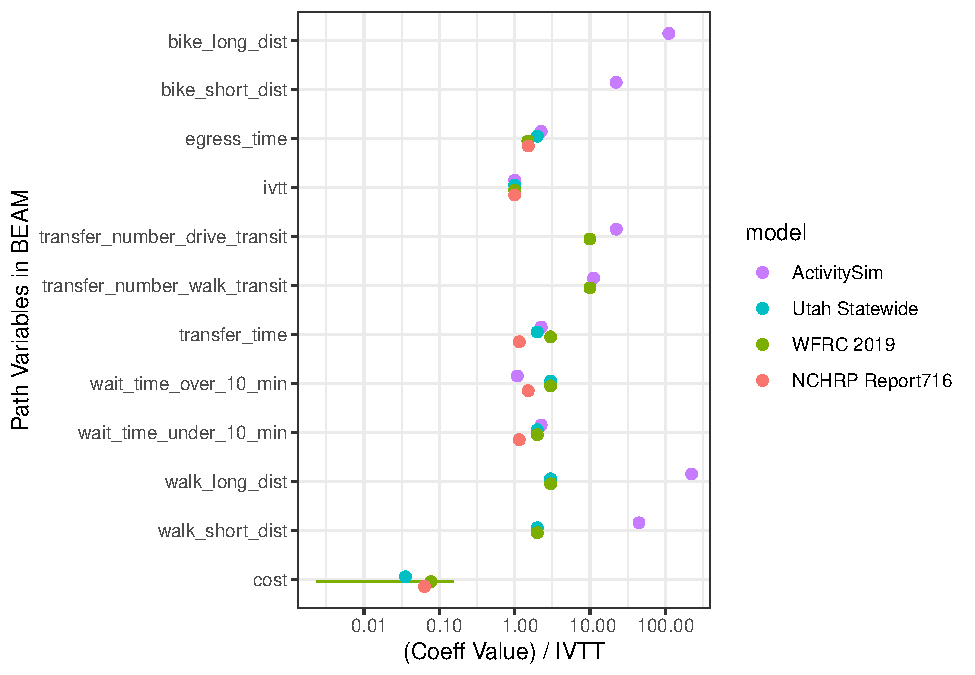
\includegraphics{thesis_files/figure-latex/hbw-1} 

}

\caption{Home-based work mode choice path coefficients model comparison.}\label{fig:hbw}
\end{figure}

Figure \ref{fig:hbs} shows the comparison of the path utility parameter values between all four models for home-based school trips. Similar to the home-based work analysis, for the egress time, ivtt, transfer time, and the wait times, ActivitySim seems to use a very similar coefficient value as the other three models. Again, the largest discrepancy exists with short and long walking distances. Since this is simply a difference between how walk distance is modeled, the discrepancy is ignored. In addition, the other three models did not have information on number of transfers. As a result, there is no comparison done with number of transfers. ActivitySim's path coefficient values do not require calibration for the home-based school parameters.

\begin{figure}

{\centering 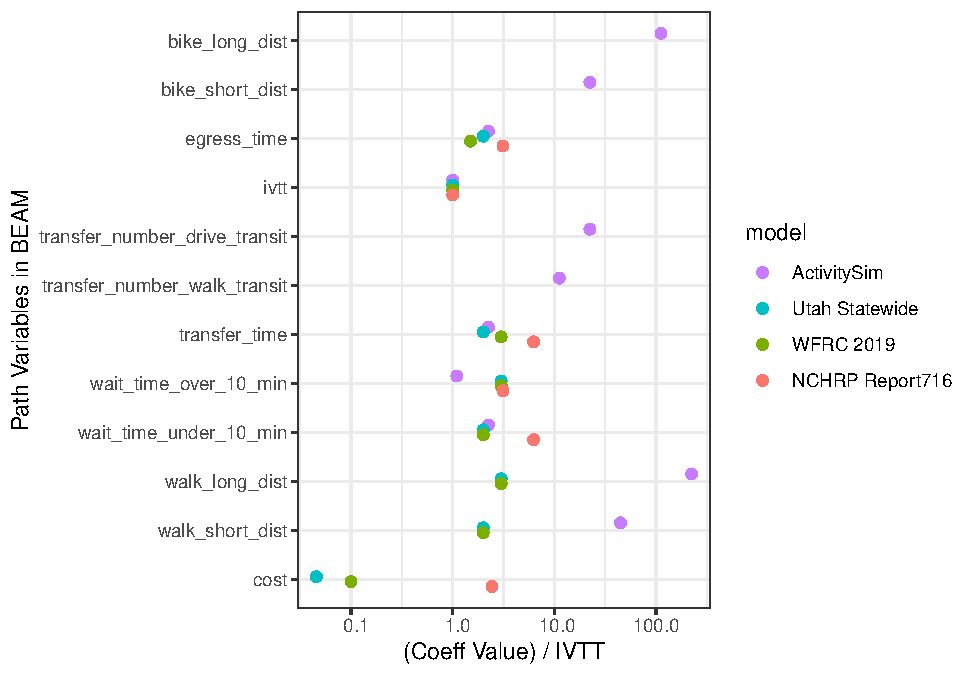
\includegraphics{thesis_files/figure-latex/hbs-1} 

}

\caption{Home-based school mode choice path coefficients model comparison.}\label{fig:hbs}
\end{figure}

Lastly, Figure \ref{fig:hbo} shows the comparison of path utility parameter values between all four models for home-based other trips. Again, besides for walk distance all variables seem to be similar between all four models. An interesting point is that for models other than ActivitySim, the cost coefficient varies greatly. Fortunately, ActivitySim bases the cost coefficient on each individual's value of time so this is not a concern. Overall, for all purpose types the coefficients used by ActivitySim are similar enough to other models that exist, and therefore do not require calibration. The ActivitySim alternative specific constants do, however, require calibration (See Section \ref{clib}).

\begin{figure}

{\centering 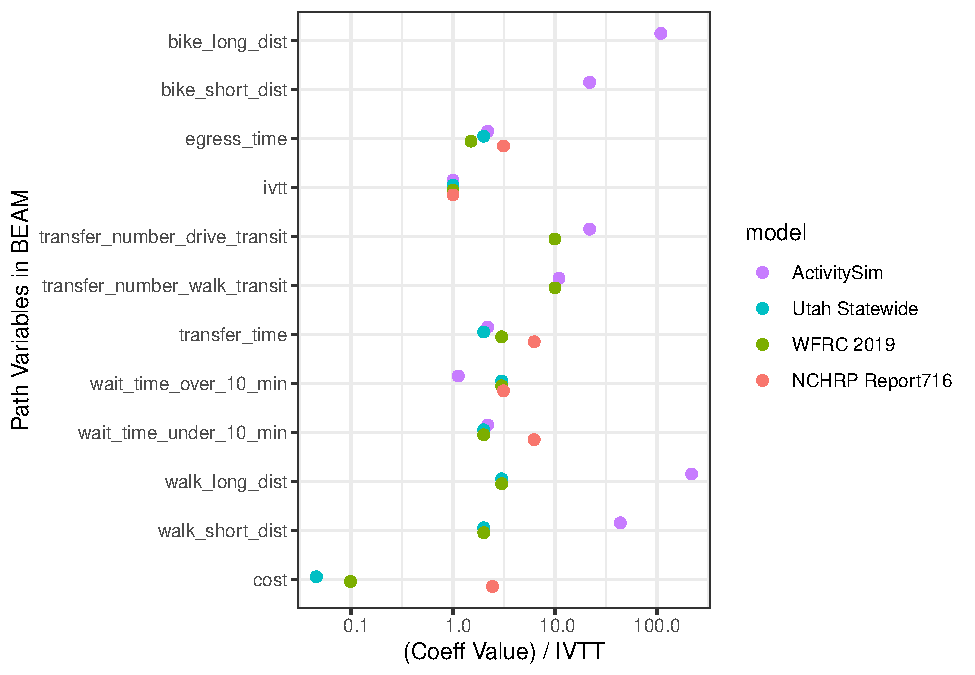
\includegraphics{thesis_files/figure-latex/hbo-1} 

}

\caption{Home-based other mode choice path coefficients model comparison.}\label{fig:hbo}
\end{figure}

After validation was completed, the last step in order to run BEAM with the case study region was to calibrate the ASC values of the mode choice model. BEAM calibration was completed by iteratively updating the ASC values using Equation \eqref{eq:eqcalib}. The number of trips totaled by tour purpose, auto ownership, and modal alternative were compared between the BEAM results and the ActivitySim results and used to adjust each ASC value. After 15 iterations of Equation \eqref{eq:eqcalib} were completed on the ASC values, the BEAM trip values were within a reasonable range to the ActivitySim target shares. Figure \ref{fig:fig-beam-calib} shows the progress of the calibration targets with the final shares after each iteration.

\begin{equation}
  NewASC = OldASC + ln(\frac{Trips_{ASIM}}{Trips_{BEAM}}) \label{eq:eqcalib}
\end{equation}

\begin{figure}

{\centering 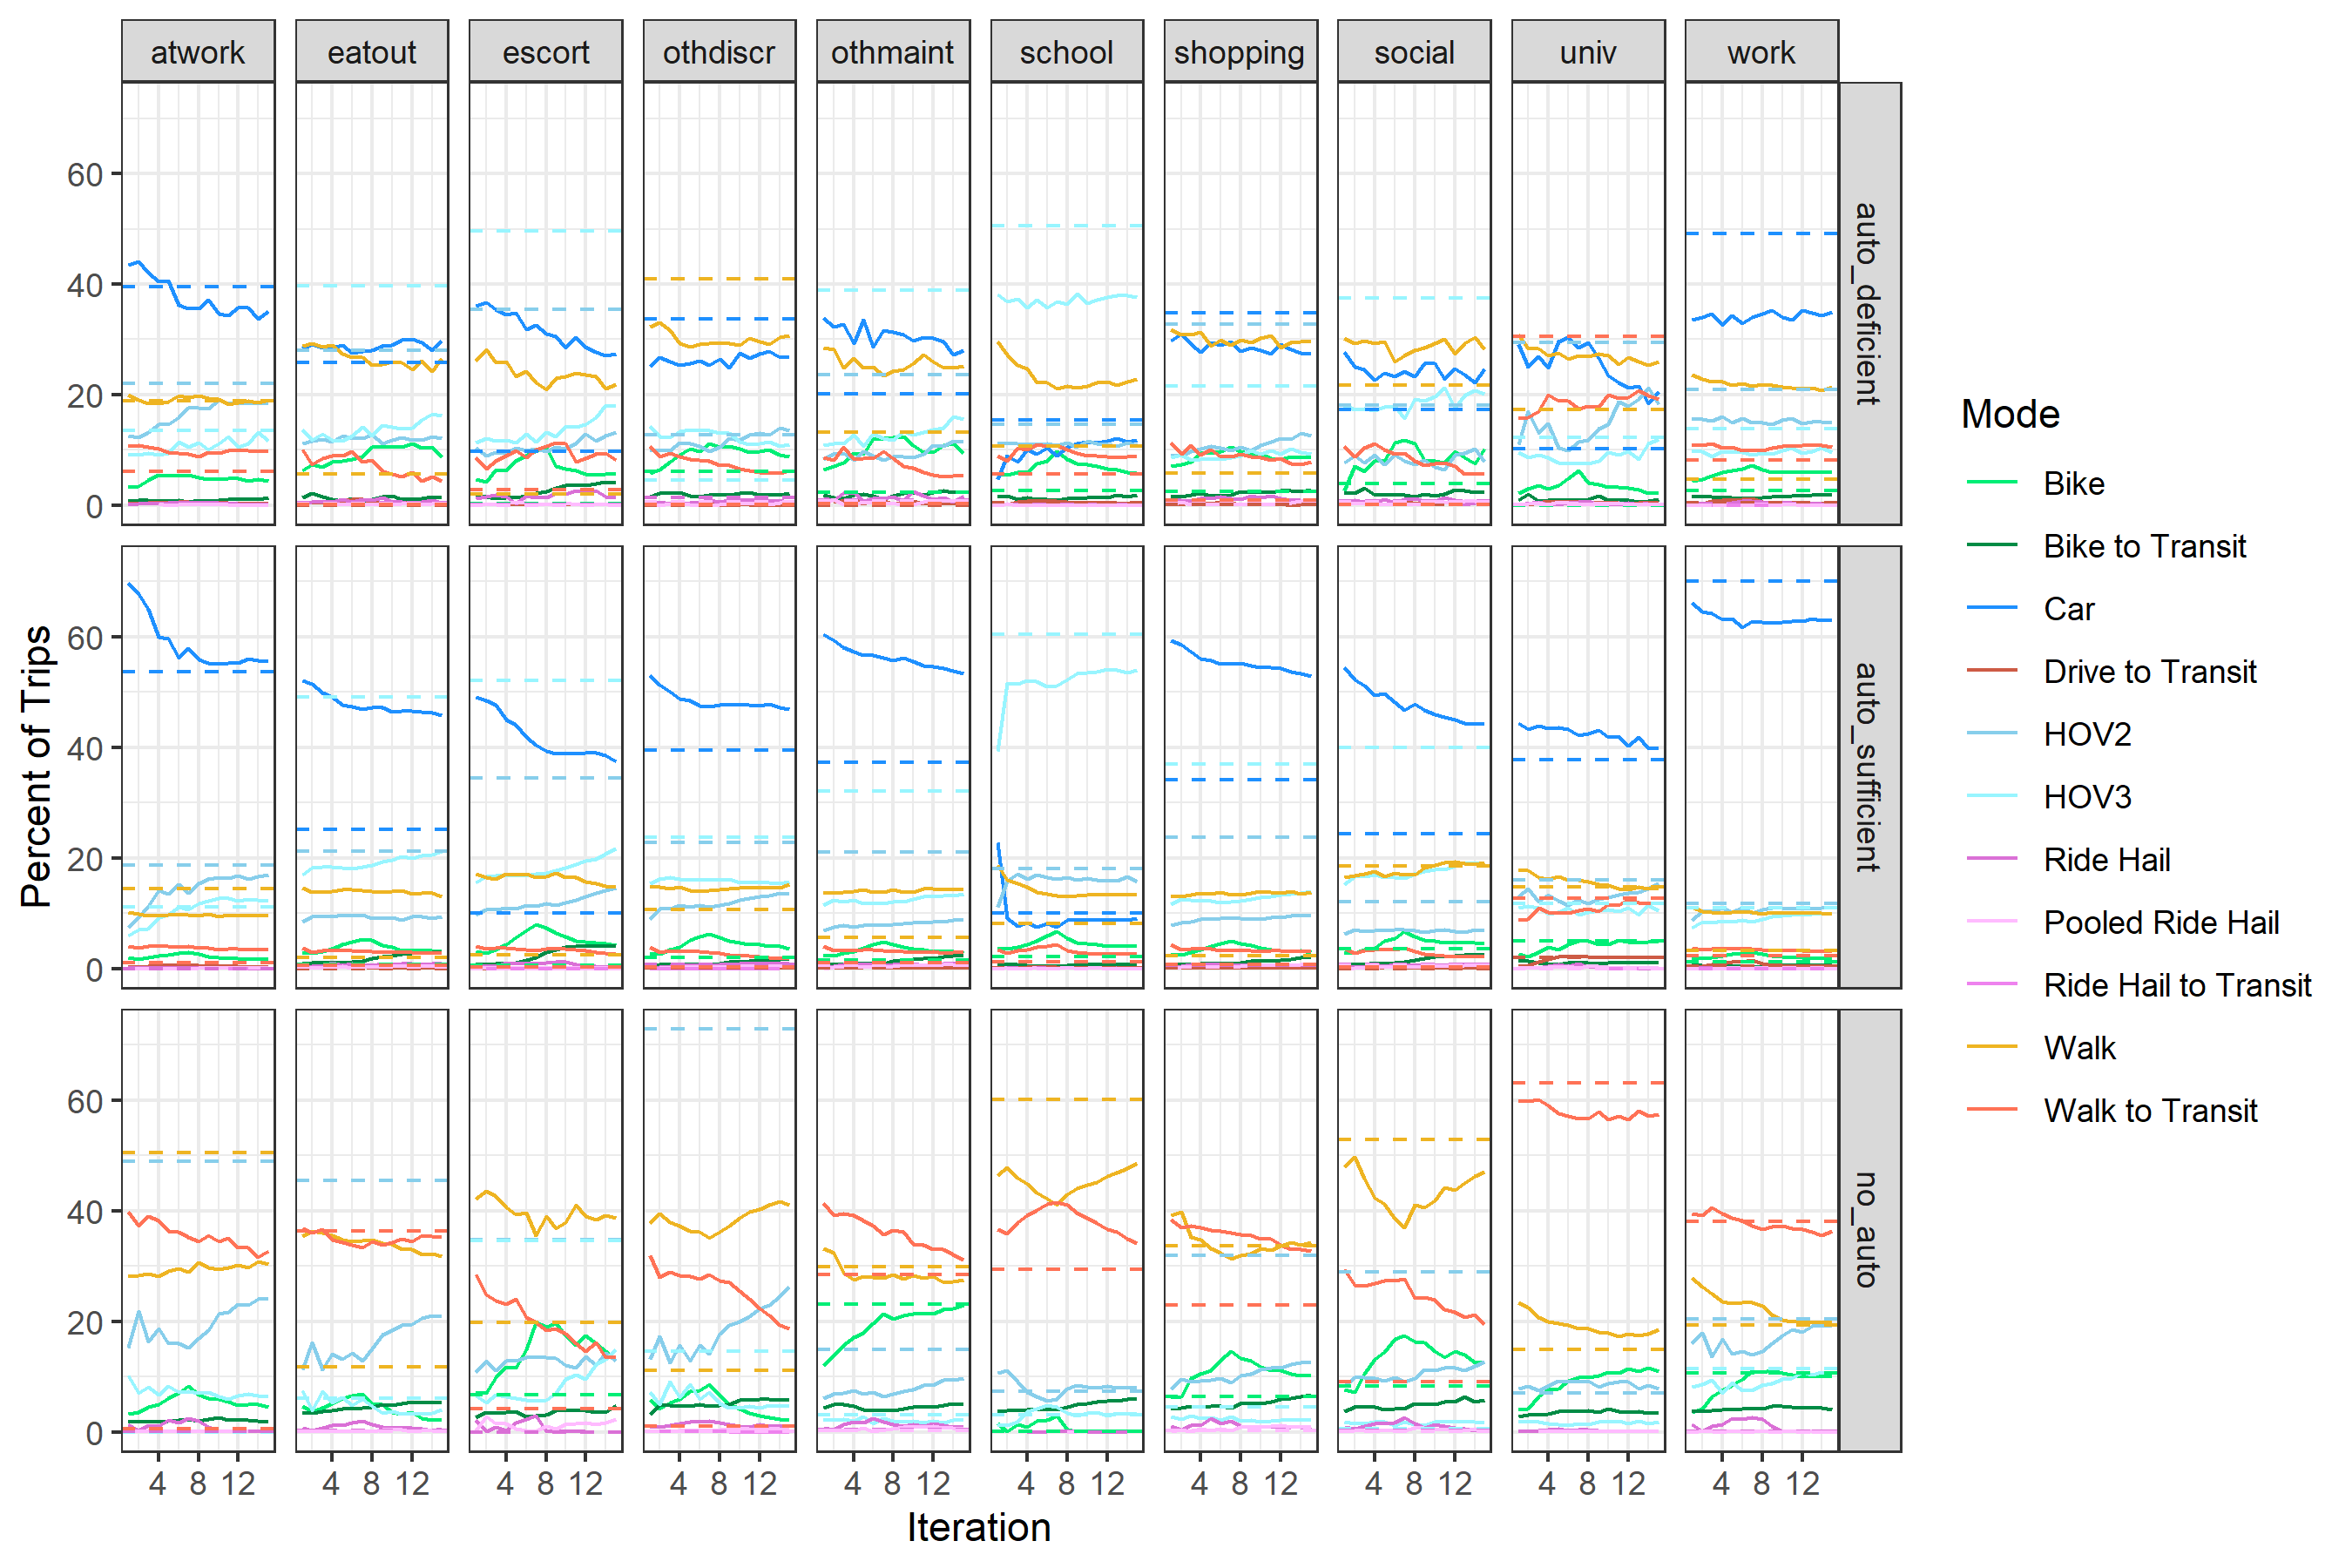
\includegraphics[width=1\linewidth]{pics/BeamCalib} 

}

\caption{BEAM mode choice ASC calibration}\label{fig:fig-beam-calib}
\end{figure}

\hypertarget{case-study-scenarios}{%
\section{Case Study Scenarios}\label{case-study-scenarios}}

After BEAM validation and BEAM calibration were completed for the case study region, a series of different BEAM scenarios were run. Specifically, 10 different experiments were conducted, each with a unique ActivitySim-to-BEAM mode choice combination. Table \ref{tab:tbexperiments} provides a short description of the 10 different scenarios.

\begin{table}

\caption{\label{tab:tbexperiments}ActivitySim - BEAM Mode Choice Combination Scenarios}
\centering
\resizebox{\linewidth}{!}{
\begin{tabular}[t]{>{\raggedright\arraybackslash}p{4em}>{\raggedright\arraybackslash}p{8em}>{\raggedright\arraybackslash}p{8em}>{\raggedright\arraybackslash}p{8em}>{\raggedright\arraybackslash}p{8em}>{\raggedright\arraybackslash}p{25em}}
\toprule
Scenario Number & Scenario Name & ActivitySim Mode Options & BEAM Mode Options & BEAM Utility Variables & Scenario Description\\
\midrule
1 & wRH-None & All Modes & No Modes & N/A & BEAM run using plans that include ride hail modes; mode innovation is turned off / mode choice remains static\\
2 & wRH-AllModes-AllVars & All Modes & All Modes & Path, Person, Location & BEAM run using ActivitySim output plans that include ride hail; all variables are used in the utility equation; all modes are available for selection\\
3 & wRH-AllModes-PathVars & All Modes & All Modes & Path & BEAM run using ActivitySim output plans that include ride hail; only path variables are used in the utility equation; all modes are available for selection\\
4 & wRH-RHModes-AllVars & All Modes & Ride Hail Modes Only & Path, Person, Location & BEAM run using ActivitySim output plans that include ride hail; all variables are used in the utility equation; mode innovation is turned off for all trips except non-car trips, which have the option to change to ride hail\\
5 & wRH-RHModes-PathVars & All Modes & Ride Hail Modes Only & Path & BEAM run using ActivitySim output plans that include ride hail; only path varibales are used in the utility equation; mode innovation is turned off for all trips except non-car trips, which have the option to change to ride hail\\
\addlinespace
6 & noRH-None & All Modes except Ride Hail & No Modes & N/A & BEAM run using ActivitySim output plans that don't include ride hail; mode innovation is turned off / mode choice remains static\\
7 & noRH-AllModes-AllVars & All Modes except Ride Hail & All Modes & Path, Person, Location & BEAM run using ActivitySim output plans that don't include ride hail; all variables are used in the utility equation; all modes are available for selection\\
8 & noRH-AllModes-PathVars & All Modes except Ride Hail & All Modes & Path & BEAM run using ActivitySim output plans that don't include ride hail; only path variables are used in the utility equation; all modes are available for selection\\
9 & noRH-RHModes-AllVars & All Modes except Ride Hail & Ride Hail Modes Only & Path, Person, Location & BEAM run using ActivitySim output plans that don't include ride hail; all variables are used in the utility equation; mode innovation is turned off for all trips except non-car trips, which have the option to change to ride hail\\
10 & noRH-RHModes-PathVars & All Modes except Ride Hail & Ride Hail Modes Only & Path & BEAM run using ActivitySim output plans that don't include ride hail; only path variables are used in the utility equation; mode innovation is turned off for all trips except non-car trips, which have the option to change to ride hail\\
\bottomrule
\end{tabular}}
\end{table}

Three different mode choice adjustments help describe the setup of each experiment. The first descriptor references how ActivitySim's modes were configured, which in Table \ref{tab:tbexperiments} is labeled as ``ActivitySim Mode Options''. Only two options are available: ``All Modes'' and ``All Modes except Ride Hail''. To explain, ActivitySim was run two times, one with ride hail alternatives turned on and one with ride hail turned off. In other words, the ride hail nesting option as shown in Figure \ref{fig-asim-nest} existed in one run of ActivitySim (``All Modes''), whereas in the other it did not (``All Modes except Ride Hail''). Since the daily activity plans generated by ActivitySim were converted to BEAM inputs, this descriptor also explains the initial mode choice selections for all trips entered into BEAM. Two different plans files were used to running BEAM: one plans file included some trips with ride hail modes whereas the other plans file included no trips with ride hail modes. By creating this distinction, we hope to better understand how heavily a multiagent simulation prioritizes ride hail as opposed to an activity-based model.

The second descriptor present in Table \ref{tab:tbexperiments} is labeled as ``BEAM Mode Options'' and explains the modal alternatives available for choice within BEAM. Three different variations were used: ``No Modes'', ``All Modes'', ``Ride Hail Modes Only''. The ``No Modes'' category represents a run of BEAM where all modal innovation was turned off. This means that no mode choice was available, and the modes from the initial input plans remained constant across each iteration. The ``All Modes'' category however, represents a run of BEAM where modal innovation was turned on, and all modal alternatives were available for choice. This meant that within-day replanning as well as across-day replanning was turned on, and agents could change their trip modes to maximize their utility. Lastly, the ``Ride Hail Modes Only'' category represented a run of BEAM where modal innovation was partially turned off. All trips that originally took car or carpool modes had modal innovation turned off; their modes were locked. All trips that originally took walk-transit or drive-transit modes, however, were given the option to switch to ride hail transit. Also, all walk modes were given the option to switch to ride hail. ``Ride Hail Modes Only'' represented the version of BEAM where ride hail and ride hail transit modes were given to non-car dependent agents. Overall, by using different mode choice structures within BEAM, we hope to better understand how altering available modal alternatives affects ride hail service capabilities.

Finally, the third descriptor present in Table \ref{tab:tbexperiments} is labeled as ``BEAM Utility Variables'' and explains which utility variables were used to calculate modal utility. Three difference variations were present: ``N/A'', ``Path, Person, Location'', and ``Path''. The ``N/A'' option means no utility parameters were used in determining mode choice, because modal innovation as turned off completely. The ``Path, Person, Location'' option represented the version of BEAM that used all utility parameter types to calculate the mode choice utility. As ActivitySim uses path, person, and location type variables to determining modes, this version of BEAM also uses all three types of variables. Section \ref{meth-beam-link} describes how BEAM was configured to use all these variable types. The ``Path'' option represented the version of BEAM that only used path type utility parameters to calculate mode choice utility; the location and person type variables were not used. By altering which variables were used in the utility equation, We hope to better understand the effect different types of utility parameters have on mode choice and ride hail service capabilities.

Overall, we ran 10 different scenarios each with a slightly different ActivitySim-to-BEAM mode choice combination. Each scenario is built from which modes were included in the input plans, which modal alternatives were available for choice, and which utility parameter types were used to calculate the mode choice utility. By altering these three different mode choice characteristics, we hope to better understand the affect a linked activity-based model and multiagent simulation have on the service capabilities of a novel mode.

\hypertarget{results}{%
\chapter{Results}\label{results}}

\hypertarget{table}{%
\section{Table}\label{table}}

\hypertarget{discussion}{%
\chapter{Discussion}\label{discussion}}

\hypertarget{conclusions}{%
\chapter{Conclusions}\label{conclusions}}

`r
\# \{=latex\} for thesis
\# \{\} for elsevier'

\cleardoublepage
    \bookmarksetupnext{level=part}
    \phantomsection
    \addcontentsline{toc}{chapter}{References}
    \begin{centering}
    REFERENCES\\
    \vskip 1 \baselineskip
    \end{centering}
    

\hypertarget{refs}{}
\begin{CSLReferences}{1}{0}
\leavevmode\vadjust pre{\hypertarget{ref-rsg21}{}}%
{``ActivitySim: An Advanced Activity-Based Travel Demand Model Built by and for Users.''} 2021. \emph{RSG}. \url{https://rsginc.com/activitysim-white-paper/\#advanced-activity-based-travel-demand-model}.

\leavevmode\vadjust pre{\hypertarget{ref-adler05}{}}%
Adler, Jeffrey L, Goutam Satapathy, Vikram Manikonda, Betty Bowles, and Victor J Blue. 2005. {``A Multi-Agent Approach to Cooperative Traffic Management and Route Guidance.''} \emph{Transportation Research Part B: Methodological} 39 (4): 297--318.

\leavevmode\vadjust pre{\hypertarget{ref-agrc}{}}%
AGRC. 2021. \emph{Automated Geographic Reference Center}. \url{https://gis.utah.gov/}.

\leavevmode\vadjust pre{\hypertarget{ref-amblard15}{}}%
Amblard, Frédéric, Eric Daudé, Benoît Gaudou, Arnaud Grignard, Guillaume Hutzler, Christophe Lang, Nicolas Marilleau, Jean-Marc Nicod, David Sheeren, and Patrick Taillandier. 2015. {``Introduction to NetLogo.''} In \emph{Agent-Based Spatial Simulation with Netlogo}, 75--123. Elsevier.

\leavevmode\vadjust pre{\hypertarget{ref-bazghandi12}{}}%
Bazghandi, Ali. 2012. {``Techniques, Advantages and Problems of Agent Based Modeling for Traffic Simulation.''} \emph{International Journal of Computer Science Issues (IJCSI)} 9 (1): 115.

\leavevmode\vadjust pre{\hypertarget{ref-beam}{}}%
BEAM. 2022. \emph{Behavior, Energy, Autonomy, and Mobility}. Lawrence Berkeley National Laboratory the UC Berkeley Institute for Transportation Studies. \url{https://beam.readthedocs.io/en/develop/users.html}.

\leavevmode\vadjust pre{\hypertarget{ref-becker20}{}}%
Becker, Henrik, Milos Balac, Francesco Ciari, and Kay W Axhausen. 2020. {``Assessing the Welfare Impacts of Shared Mobility and Mobility as a Service (MaaS).''} \emph{Transportation Research Part A: Policy and Practice} 131: 228--43.

\leavevmode\vadjust pre{\hypertarget{ref-biehl19}{}}%
Biehl, Alec, Alireza Ermagun, and Amanda Stathopoulos. 2019. {``Utilizing Multi-Stage Behavior Change Theory to Model the Process of Bike Share Adoption.''} \emph{Transport Policy} 77: 30--45.

\leavevmode\vadjust pre{\hypertarget{ref-bowman98}{}}%
Bowman, John Lawrence. 1998. {``The Day Activity Schedule Approach to Travel Demand Analysis.''} PhD thesis, Massachusetts Institute of Technology.

\leavevmode\vadjust pre{\hypertarget{ref-nchrp}{}}%
Cambridge Systematics, Inc., Inc. Vanasse Hangen Brustlin, Gallop Corporation, Chandra R. Bhat, LLC Shapiro Transportation Consulting, and PLLC Martin/Alexiou/Bryson. 2012. {``Travel Demand Forecasting: Parameters and Techniques.''} In \emph{NCHRP Report 716}, 55--60. Transportation Research Board.

\leavevmode\vadjust pre{\hypertarget{ref-campbell16}{}}%
Campbell, Andrew A, Christopher R Cherry, Megan S Ryerson, and Xinmiao Yang. 2016. {``Factors Influencing the Choice of Shared Bicycles and Shared Electric Bikes in Beijing.''} \emph{Transportation Research Part C: Emerging Technologies} 67: 399--414.

\leavevmode\vadjust pre{\hypertarget{ref-cetin02}{}}%
Cetin, Nurhan, Kai Nagel, Bryan Raney, and Andreas Voellmy. 2002. {``Large-Scale Multi-Agent Transportation Simulations.''} \emph{Computer Physics Communications} 147 (1-2): 559--64.

\leavevmode\vadjust pre{\hypertarget{ref-cho22}{}}%
Cho, Shin-Hyung, and DongHwa Shin. 2022. {``Estimation of Route Choice Behaviors of Bike-Sharing Users as First-and Last-Mile Trips for Introduction of Mobility-as-a-Service (MaaS).''} \emph{KSCE Journal of Civil Engineering}, 1--12.

\leavevmode\vadjust pre{\hypertarget{ref-ciari16}{}}%
Ciari, Francesco, Milos Balac, and Kay W Axhausen. 2016. {``Modeling Carsharing with the Agent-Based Simulation MATSim: State of the Art, Applications, and Future Developments.''} \emph{Transportation Research Record} 2564 (1): 14--20.

\leavevmode\vadjust pre{\hypertarget{ref-r5}{}}%
Conveyal. 2022. \emph{R5: Rapid Realistic Routing on Real-World and Reimagined Networks}. \url{https://github.com/conveyal/r5}.

\leavevmode\vadjust pre{\hypertarget{ref-dean21}{}}%
Dean, Matthew D, and Kara M Kockelman. 2021. {``Spatial Variation in Shared Ride-Hail Trip Demand and Factors Contributing to Sharing: Lessons from Chicago.''} \emph{Journal of Transport Geography} 91: 102944.

\leavevmode\vadjust pre{\hypertarget{ref-dia02}{}}%
Dia, Hussein. 2002. {``An Agent-Based Approach to Modelling Driver Route Choice Behaviour Under the Influence of Real-Time Information.''} \emph{Transportation Research Part C: Emerging Technologies} 10 (5-6): 331--49.

\leavevmode\vadjust pre{\hypertarget{ref-djavadian17}{}}%
Djavadian, Shadi, and Joseph YJ Chow. 2017. {``An Agent-Based Day-to-Day Adjustment Process for Modeling `Mobility as a Service'with a Two-Sided Flexible Transport Market.''} \emph{Transportation Research Part B: Methodological} 104: 36--57.

\leavevmode\vadjust pre{\hypertarget{ref-dong20}{}}%
Dong, Xiaoxia. 2020. {``Trade Uber for the Bus?''} \emph{Journal of the American Planning Association} 86 (2): 222--35.

\leavevmode\vadjust pre{\hypertarget{ref-fujii17}{}}%
Fujii, Hideki, Hideaki Uchida, and Shinobu Yoshimura. 2017. {``Agent-Based Simulation Framework for Mixed Traffic of Cars, Pedestrians and Trams.''} \emph{Transportation Research Part C: Emerging Technologies} 85: 234--48.

\leavevmode\vadjust pre{\hypertarget{ref-gali08}{}}%
Gali, Emmanuel, Stephan Eidenbenz, Sue Mniszewski, Leticia Cuellar, and Christof Teuscher. 2008. {``ActivitySim: Large-Scale Agent Based Activity Generation for Infrastructure Simulation,''} January. \url{https://www.osti.gov/biblio/960770}.

\leavevmode\vadjust pre{\hypertarget{ref-gomes21}{}}%
Gomes, Viviani Antunes, MUC CALDAS, and Cira Souza Pitombo. 2021. {``An Investigation of Trip-Chaining Behaviour Based on Activity Participation, Socioeconomic Variables and Aggregated Characteristics of Modal Alternatives.''} \emph{Revista Transportes} 29 (1): 21--41.

\leavevmode\vadjust pre{\hypertarget{ref-hasnine21}{}}%
Hasnine, Md Sami, and Khandker Nurul Habib. 2021. {``Tour-Based Mode Choice Modelling as the Core of an Activity-Based Travel Demand Modelling Framework: A Review of State-of-the-Art.''} \emph{Transport Reviews} 41 (1): 5--26.

\leavevmode\vadjust pre{\hypertarget{ref-horl19}{}}%
Hörl, Sebastian, Miloš Balać, and Kay W Axhausen. 2019. {``Pairing Discrete Mode Choice Models and Agent-Based Transport Simulation with MATSim.''} In \emph{2019 TRB Annual Meeting Online}, 19--02409. Transportation Research Board.

\leavevmode\vadjust pre{\hypertarget{ref-horl19b}{}}%
Hörl, Sebastian, Claudio Ruch, Felix Becker, Emilio Frazzoli, and Kay W Axhausen. 2019. {``Fleet Operational Policies for Automated Mobility: A Simulation Assessment for Zurich.''} \emph{Transportation Research Part C: Emerging Technologies} 102: 20--31.

\leavevmode\vadjust pre{\hypertarget{ref-hosseinzadeh21}{}}%
Hosseinzadeh, Aryan, Majeed Algomaiah, Robert Kluger, and Zhixia Li. 2021. {``Spatial Analysis of Shared e-Scooter Trips.''} \emph{Journal of Transport Geography} 92: 103016.

\leavevmode\vadjust pre{\hypertarget{ref-hyland18}{}}%
Hyland, Michael, Zihan Hong, Helen Karla Ramalho de Farias Pinto, and Ying Chen. 2018. {``Hybrid Cluster-Regression Approach to Model Bikeshare Station Usage.''} \emph{Transportation Research Part A: Policy and Practice} 115: 71--89.

\leavevmode\vadjust pre{\hypertarget{ref-kamel19}{}}%
Kamel, Joseph, Reza Vosooghi, Jakob Puchinger, Feirouz Ksontini, and Göknur Sirin. 2019. {``Exploring the Impact of User Preferences on Shared Autonomous Vehicle Modal Split: A Multi-Agent Simulation Approach.''} \emph{Transportation Research Procedia} 37: 115--22.

\leavevmode\vadjust pre{\hypertarget{ref-kang21}{}}%
Kang, Shuqing, Aupal Mondal, Aarti C Bhat, and Chandra R Bhat. 2021. {``Pooled Versus Private Ride-Hailing: A Joint Revealed and Stated Preference Analysis Recognizing Psycho-Social Factors.''} \emph{Transportation Research Part C: Emerging Technologies} 124: 102906.

\leavevmode\vadjust pre{\hypertarget{ref-knapen21}{}}%
Knapen, Luk, Muhammad Adnan, Bruno Kochan, Tom Bellemans, Marieke van der Tuin, Han Zhou, and Maaike Snelder. 2021. {``An Activity Based Integrated Approach to Model Impacts of Parking, Hubs and New Mobility Concepts.''} \emph{Procedia Computer Science} 184: 428--37.

\leavevmode\vadjust pre{\hypertarget{ref-nate}{}}%
Lant, Nathan John. 2021. {``Estimation and Simulation of Daily Activity Patterns for Individuals Using Wheelchairs.''} PhD thesis, Brigham Young University.

\leavevmode\vadjust pre{\hypertarget{ref-lazarus20}{}}%
Lazarus, Jessica, Jean Carpentier Pourquier, Frank Feng, Henry Hammel, and Susan Shaheen. 2020. {``Micromobility Evolution and Expansion: Understanding How Docked and Dockless Bikesharing Models Complement and Compete--a Case Study of San Francisco.''} \emph{Journal of Transport Geography} 84: 102620.

\leavevmode\vadjust pre{\hypertarget{ref-leeb21}{}}%
Lee, Hyukseong, Kwangho Baek, Jin-Hyuk Chung, and Jinhee Kim. 2021. {``Factors Affecting Heterogeneity in Willingness to Use e-Scooter Sharing Services.''} \emph{Transportation Research Part D: Transport and Environment} 92: 102751.

\leavevmode\vadjust pre{\hypertarget{ref-lee21}{}}%
Lee, Mina, Joseph YJ Chow, Gyugeun Yoon, and Brian Yueshuai He. 2021. {``Forecasting e-Scooter Substitution of Direct and Access Trips by Mode and Distance.''} \emph{Transportation Research Part D: Transport and Environment} 96: 102892.

\leavevmode\vadjust pre{\hypertarget{ref-li18b}{}}%
Li, Qing, Feixiong Liao, Harry JP Timmermans, Haijun Huang, and Jing Zhou. 2018. {``Incorporating Free-Floating Car-Sharing into an Activity-Based Dynamic User Equilibrium Model: A Demand-Side Model.''} \emph{Transportation Research Part B: Methodological} 107: 102--23.

\leavevmode\vadjust pre{\hypertarget{ref-li18}{}}%
Li, Weibo, and Maria Kamargianni. 2018. {``Providing Quantified Evidence to Policy Makers for Promoting Bike-Sharing in Heavily Air-Polluted Cities: A Mode Choice Model and Policy Simulation for Taiyuan-China.''} \emph{Transportation Research Part A: Policy and Practice} 111: 277--91.

\leavevmode\vadjust pre{\hypertarget{ref-li20}{}}%
Li, Yuanyuan, Yang Liu, and Jun Xie. 2020. {``A Path-Based Equilibrium Model for Ridesharing Matching.''} \emph{Transportation Research Part B: Methodological} 138: 373--405.

\leavevmode\vadjust pre{\hypertarget{ref-macfarlane21}{}}%
Macfarlane, Gregory S, Nathan J Lant, et al. 2021. {``Estimation and Simulation of Daily Activity Patterns for Individuals Using Wheelchairs.''} Utah. Dept. of Transportation. Division of Research.

\leavevmode\vadjust pre{\hypertarget{ref-mahmoudi21}{}}%
Mahmoudi, Monirehalsadat, Lu (Carol) Tong, Venu M. Garikapati, Ram M. Pendyala, and Xuesong Zhou. 2021. {``How Many Trip Requests Could We Support? An Activity-Travel Based Vehicle Scheduling Approach.''} \emph{Transportation Research Part C: Emerging Technologies} 128. https://doi.org/\url{https://doi.org/10.1016/j.trc.2021.103222}.

\leavevmode\vadjust pre{\hypertarget{ref-mckenzie19}{}}%
McKenzie, Grant. 2019. {``Spatiotemporal Comparative Analysis of Scooter-Share and Bike-Share Usage Patterns in Washington, DC.''} \emph{Journal of Transport Geography} 78: 19--28.

\leavevmode\vadjust pre{\hypertarget{ref-mo22}{}}%
Mo, Dong, Xiqun Michael Chen, and Junlin Zhang. 2022. {``Modeling and Managing Mixed on-Demand Ride Services of Human-Driven Vehicles and Autonomous Vehicles.''} \emph{Transportation Research Part B: Methodological} 157: 80--119.

\leavevmode\vadjust pre{\hypertarget{ref-moeckel20}{}}%
Moeckel, Rolf, Nico Kuehnel, Carlos Llorca, Ana Tsui Moreno, and Hema Rayaprolu. 2020. {``Agent-Based Simulation to Improve Policy Sensitivity of Trip-Based Models.''} \emph{Journal of Advanced Transportation} 2020.

\leavevmode\vadjust pre{\hypertarget{ref-mtc12}{}}%
MTC. 2012. \emph{Travel Model Development: Calibration and Validation Technical Report}. Metropolitan Transportation Commission with Parsons Brinckerhoff, Inc.

\leavevmode\vadjust pre{\hypertarget{ref-muhammad19}{}}%
Muhammad, Hafiz, Ahsan IQBAL, Muhammad ADNAN, Bruno KOCHAN, Tom BELLEMANS, and Davy JANSSENS. 2019. {``Incorporating MaaS Concept into an Operational Activity-Based Modelling Platform.''} In.

\leavevmode\vadjust pre{\hypertarget{ref-nayak22}{}}%
Nayak, Suchismita, and Debapratim Pandit. 2022. {``Activity-Based Model: Requisite for a New Travel Demand Forecasting Approach for India.''} In \emph{Proceedings of the Fifth International Conference of Transportation Research Group of India}, 109--21. Springer.

\leavevmode\vadjust pre{\hypertarget{ref-neutens08}{}}%
Neutens, Tijs, Tim Schwanen, Frank Witlox, and Philippe De Maeyer. 2008. {``My Space or Your Space? Towards a Measure of Joint Accessibility.''} \emph{Computers, Environment and Urban Systems} 32 (5): 331--42.

\leavevmode\vadjust pre{\hypertarget{ref-nguyen22}{}}%
Nguyen, Tri K, Nam H Hoang, and Hai L Vu. 2022. {``A Unified Activity-Based Framework for One-Way Car-Sharing Services in Multi-Modal Transportation Networks.''} \emph{Transportation Research Part E: Logistics and Transportation Review} 157: 102551.

\leavevmode\vadjust pre{\hypertarget{ref-pendyala17}{}}%
Pendyala, Ram M, Daehyun You, Venu M Garikapati, Karthik C Konduri, and Xuesong Zhou. 2017. {``Paradigms for Integrated Modeling of Activity-Travel Demand and Network Dynamics in an Era of Dynamic Mobility Management.''}

\leavevmode\vadjust pre{\hypertarget{ref-philip13}{}}%
Philip, Milimol, T Sreelatha, and Soosan George. 2013. {``Activity Based Travel Behavioural Study and Mode Choice Modelling.''} \emph{Int J Innov Res Sci Eng Technol} 2 (1): 181--90.

\leavevmode\vadjust pre{\hypertarget{ref-popsim}{}}%
PopulationSim. 2021. \emph{An Open Platform for Population Synthesis} (version 0.5). \url{https://activitysim.github.io/populationsim/}.

\leavevmode\vadjust pre{\hypertarget{ref-reck21}{}}%
Reck, Daniel J, He Haitao, Sergio Guidon, and Kay W Axhausen. 2021. {``Explaining Shared Micromobility Usage, Competition and Mode Choice by Modelling Empirical Data from Zurich, Switzerland.''} \emph{Transportation Research Part C: Emerging Technologies} 124: 102947.

\leavevmode\vadjust pre{\hypertarget{ref-rsg16}{}}%
RSG. 2016. \emph{Pricing and Travel Time Reliability Enhancements in the SANDAG Activity-Based Travel Model: Final Report}.

\leavevmode\vadjust pre{\hypertarget{ref-sanchez19}{}}%
Sánchez, Pedro, Denis Pato, Gabriel Martín, et al. 2019. {``CTRANSPORT: Multi-Agent-Based Simulation.''}

\leavevmode\vadjust pre{\hypertarget{ref-shiftan00}{}}%
Shiftan, Yoram. 2000. {``The Advantage of Activity-Based Modelling for Air-Quality Purposes: Theory Vs Practice and Future Needs.''} \emph{Innovation: The European Journal of Social Science Research} 13 (1): 95--110.

\leavevmode\vadjust pre{\hypertarget{ref-shimizu13}{}}%
Shimizu, Shota, Kenju Akai, and Nariaki Nishino. 2013. {``Modeling and Multi-Agent Simulation of Bicycle Sharing.''} In \emph{International Conference on Serviceology}, 39--46. Springer.

\leavevmode\vadjust pre{\hypertarget{ref-siebers08}{}}%
Siebers, Peer-Olaf, and Uwe Aickelin. 2008. {``Introduction to Multi-Agent Simulation.''} In \emph{Encyclopedia of Decision Making and Decision Support Technologies}, 554--64. IGI Global.

\leavevmode\vadjust pre{\hypertarget{ref-song19}{}}%
Song, Mingzhu, Yi Zhang, Zuojun Max Shen, Meng Li, and Zhenning Dong. 2019. {``Mode Shift from Car to Bike Shared: A Travel-Mode Choice Model.''} In \emph{CICTP 2019}, 2398--2410.

\leavevmode\vadjust pre{\hypertarget{ref-soo09}{}}%
Soo (Kum Lin, Joyce). 2009. \emph{Towards a Multi-Activity Multi-Erson Accessibility Measure}. Faculty of Geosciences, Utrecht University.

\leavevmode\vadjust pre{\hypertarget{ref-tchappi18}{}}%
Tchappi, Igor Haman, Stéphane Galland, Vivient Corneille Kamla, and Jean Claude Kamgang. 2018. {``A Brief Review of Holonic Multi-Agent Models for Traffic and Transportation Systems.''} \emph{Procedia Computer Science} 134: 137--44.

\leavevmode\vadjust pre{\hypertarget{ref-tuli21}{}}%
Tuli, Farzana Mehzabin, Suman Mitra, and Mariah B Crews. 2021. {``Factors Influencing the Usage of Shared e-Scooters in Chicago.''} \emph{Transportation Research Part A: Policy and Practice} 154: 164--85.

\leavevmode\vadjust pre{\hypertarget{ref-tzouras22}{}}%
Tzouras, Panagiotis G, Lambros Mitropoulos, Eirini Stavropoulou, Eleni Antoniou, Katerina Koliou, Christos Karolemeas, Antonis Karaloulis, et al. 2022. {``Agent-Based Models for Simulating e-Scooter Sharing Services: A Review and a Qualitative Assessment.''} \emph{International Journal of Transportation Science and Technology}.

\leavevmode\vadjust pre{\hypertarget{ref-utahstate}{}}%
UDOT. 2021. \emph{Utah State Travel Demand Model}. Utah Department of Transportation.

\leavevmode\vadjust pre{\hypertarget{ref-vyas19}{}}%
Vyas, Gaurav, Pooneh Famili, Peter Vovsha, Daniel Fay, Ashish Kulshrestha, Greg Giaimo, and Rebekah Anderson. 2019. {``Incorporating Features of Autonomous Vehicles in Activity-Based Travel Demand Model for Columbus, OH.''} \emph{Transportation} 46 (6): 2081--2102.

\leavevmode\vadjust pre{\hypertarget{ref-wadud21}{}}%
Wadud, Zia, and Phani Kumar Chintakayala. 2021. {``To Own or Not to Own--That Is the Question: The Value of Owning a (Fully Automated) Vehicle.''} \emph{Transportation Research Part C: Emerging Technologies} 123: 102978.

\leavevmode\vadjust pre{\hypertarget{ref-welch20}{}}%
Welch, Timothy F, Steven R Gehrke, and Alyas Widita. 2020. {``Shared-Use Mobility Competition: A Trip-Level Analysis of Taxi, Bikeshare, and Transit Mode Choice in Washington, DC.''} \emph{Transportmetrica A: Transport Science} 16 (1): 43--55.

\leavevmode\vadjust pre{\hypertarget{ref-wfrc}{}}%
WFRC. 2019. \emph{Wasatch Front Travel Demand Model} (version v8.3.1). Wasatch Front Regional Council. \url{https://wfrc.org/programs/models-forecasting/}.

\leavevmode\vadjust pre{\hypertarget{ref-xu19}{}}%
Xu, Xiang, Hani S Mahmassani, and Ying Chen. 2019. {``Privately Owned Autonomous Vehicle Optimization Model Development and Integration with Activity-Based Modeling and Dynamic Traffic Assignment Framework.''} \emph{Transportation Research Record} 2673 (10): 683--95.

\leavevmode\vadjust pre{\hypertarget{ref-younes20}{}}%
Younes, Hannah, Zhenpeng Zou, Jiahui Wu, and Giovanni Baiocchi. 2020. {``Comparing the Temporal Determinants of Dockless Scooter-Share and Station-Based Bike-Share in Washington, DC.''} \emph{Transportation Research Part A: Policy and Practice} 134: 308--20.

\leavevmode\vadjust pre{\hypertarget{ref-zhang06}{}}%
Zhang, Junyi, and Akimasa Fujiwara. 2006. {``Representing Household Time Allocation Behavior by Endogenously Incorporating Diverse Intra-Household Interactions: A Case Study in the Context of Elderly Couples.''} \emph{Transportation Research Part B: Methodological} 40 (1): 54--74.

\leavevmode\vadjust pre{\hypertarget{ref-zhang18}{}}%
Zhang, Lei, Di Yang, Sepehr Ghader, Carlos Carrion, Chenfeng Xiong, Thomas F Rossi, Martin Milkovits, Subrat Mahapatra, and Charles Barber. 2018. {``An Integrated, Validated, and Applied Activity-Based Dynamic Traffic Assignment Model for the Baltimore-Washington Region.''} \emph{Transportation Research Record} 2672 (51): 45--55.

\leavevmode\vadjust pre{\hypertarget{ref-zhang21}{}}%
Zhang, Wenwen, Ralph Buehler, Andrea Broaddus, and Ted Sweeney. 2021. {``What Type of Infrastructures Do e-Scooter Riders Prefer? A Route Choice Model.''} \emph{Transportation Research Part D: Transport and Environment} 94: 102761.

\leavevmode\vadjust pre{\hypertarget{ref-zhou20}{}}%
Zhou, Fan, Zuduo Zheng, Jake Whitehead, Simon Washington, Robert K Perrons, and Lionel Page. 2020. {``Preference Heterogeneity in Mode Choice for Car-Sharing and Shared Automated Vehicles.''} \emph{Transportation Research Part A: Policy and Practice} 132: 633--50.

\leavevmode\vadjust pre{\hypertarget{ref-zhou19}{}}%
Zhou, Xiaolu, Mingshu Wang, and Dongying Li. 2019. {``Bike-Sharing or Taxi? Modeling the Choices of Travel Mode in Chicago Using Machine Learning.''} \emph{Journal of Transport Geography} 79: 102479.

\leavevmode\vadjust pre{\hypertarget{ref-zuniga22}{}}%
Zuniga-Garcia, Natalia, Mauricio Tec, James G Scott, and Randy B Machemehl. 2022. {``Evaluation of e-Scooters as Transit Last-Mile Solution.''} \emph{Transportation Research Part C: Emerging Technologies} 139: 103660.

\leavevmode\vadjust pre{\hypertarget{ref-zwick21}{}}%
Zwick, Felix, Nico Kuehnel, Rolf Moeckel, and Kay W Axhausen. 2021. {``Agent-Based Simulation of City-Wide Autonomous Ride-Pooling and the Impact on Traffic Noise.''} \emph{Transportation Research Part D: Transport and Environment} 90: 102673.

\end{CSLReferences}


% Index?

\end{document}
